\documentclass[11pt]{article}

\usepackage{epsf,epsfig,subfigure,latexsym,latexsym,amssymb,alltt}
\usepackage{xspace,graphicx,makeidx}
\usepackage{hyperref}

\pagestyle{headings}
\bibliographystyle{plain}

%%\setlength{\topmargin}{-0.25in}
\setlength{\headheight}{10pt}
\setlength{\headsep}{30pt}
\setlength{\oddsidemargin}{0.0in}
\setlength{\evensidemargin}{0.0in}
\setlength{\textheight}{8.5in}
\setlength{\textwidth}{6.5in}
\setlength{\footskip}{50pt}


\setlength{\parskip}{2mm}               % space between paragraphs

\def\cut{\mbox{\tt '!'/0}}

\newtheorem{example}{Example}[section]

\newenvironment{Prog}{\begin{tt}\begin{tabular}[c]{l}}{\end{tabular}\end{tt}}

\newcommand{\comment}[1]{}

\newcommand{\demo}[1]{\hspace*{1.5cm}{\tt #1}}
\newcommand{\desc}[1]{\item[{\tt #1}]\hspace*{1mm}\newline}
\newcommand{\desce}[1]{\item[{\tt #1}]}
\newcommand{\ourrepeatitem}[1]{\item[{\mbox{\tt #1}}]\ \\ \vspace*{-.35in}}
\newcommand{\ouritem}[1]{\item[{\mbox{\tt #1}}]\ \\}
\newcommand{\ournewitem}[2]{\item[{\mbox{\tt #1}}]\hspace*{\fill}{\mbox{\tt #2}}\ \\}

\newcommand{\stuff}[1]{
        \begin{minipage}{4in}
        {\tt \samepage
        \begin{tabbing}
        \hspace{8mm} \= \hspace{6mm} \= \hspace{10mm} \= \hspace{55mm} \= \kill
        #1 \hfill
        \end{tabbing}
        }
        \end{minipage}
}

\newcommand{\longline}{\noindent\rule{\textwidth}{.01in}}


\newenvironment{qrules}{\begin{quote}\tt\begin{tabular}[t]{l}}%
{\end{tabular}\end{quote}}


\newcommand{\obj}{\textit{obj}\xspace}
\newcommand{\db}[1]{\ensuremath{\mathcal{#1}}}

\newcommand{\xany}{\textsf{any}}

\newcommand{\xplus}{\ensuremath{^+}}
\newcommand{\xstar}{\ensuremath{^*}}
\newcommand{\xinv}{\ensuremath{^{-1}}}
\newcommand{\xopt}{\ensuremath{^{?}}}

\newcommand{\xto}[1]{\ensuremath{^{#1}}}
\newcommand{\xcond}[1]{\ensuremath{\textsf{if}(#1)}}
\newcommand{\xif}[1]{\ensuremath{\textsf{if}(#1)}}
\newcommand{\xmu}[1]{\ensuremath{\tcmu(#1)}}
\newcommand{\xmuif}[2]{\ensuremath{\tcmu(#1,#2)}}


\newcommand{\xconc}{\ensuremath{{\cdot}}}
\newcommand{\xor}{\ensuremath{|}}

\newcommand{\nnot}{\mbox{$\neg$}}                           % negation
\newcommand{\query}{\mbox{$\, ?\! - \, $}}                  % query
\newcommand{\impl}                                          % implication
  {\mbox{\Large $\; {\bf \leftarrow} \;$}}  
\newcommand{\isa}{\,{\bf{:}}\,}
\newcommand{\subcl}{\,{\bf{::}}\,}
\newcommand{\eq}{\ensuremath{\doteq}}                           % equation

% f-logic arrows

\newcommand{\fd}{\ensuremath{{\rightarrow}}}                   % scalar
\newcommand{\bfd}{\ensuremath{{\bullet\!\!\!\fd}}}            % " + inheritable
\newcommand{\mvd}{\ensuremath{{\rightarrow\!\!\!\!\rightarrow}}}  % multivalued
\newcommand{\bmvd}{\ensuremath{{\bullet\!\!\!\mvd}}}              % " + inheritable
\newcommand{\Fd}{\ensuremath{{\Rightarrow}}}                      % scalar signature
\newcommand{\Mvd}{\ensuremath{{\Rightarrow\!\!\!\!\Rightarrow}}}  % multiv signature



% curved f-logic arrows

\newcommand{\anyd}{\ensuremath{\leadsto}}                       % noninheritable
\newcommand{\bleadsto}{\ensuremath{\bullet\!\!\!\leadsto}}     % inheritable
\newcommand{\banyd}{\bleadsto}                              % "
\newcommand{\Leadsto}{\ensuremath{\approx}\!\!{>}}            % signature
\newcommand{\Anyd}{\Leadsto}                                % "

\newcommand{\FdConstr}{\ensuremath{\stackrel{constr}{\Fd}}}
\newcommand{\MvdConstr}{\ensuremath{\stackrel{constr}{\Mvd}}}

\newlength{\flogicindent}


\newlength{\flength}
\newlength{\counterlength}


\newcommand{\la}{\ensuremath{\,\leftarrow\,}}

\newcommand{\anon}{\_}

\newcommand{\note}[1]{\textit{[[#1]]}}
\newcommand{\nterm}[1]{\ensuremath{\langle}\textit{#1}\ensuremath{\rangle}}



\newcommand{\bs}{\ensuremath{\backslash}}
\newcommand{\FLIP}{{\mbox{\sc Flip}}\xspace}
\newcommand{\FLORA}{{\mbox{${\cal F}${\small\it LORA}\rm\emph{-2}}}\xspace}
\newcommand{\FLORAone}{{\mbox{${\cal F}${\sc lora}}}\xspace}
\newcommand{\FLORID}{{\mbox{\sc Florid}}\xspace}
\newcommand{\fl}{\mbox{F-logic}\xspace}
\newcommand{\NAF}{{$\tt\backslash +$}\xspace}


\newcommand{\consts}{\ensuremath{\mathcal{C}}}
\newcommand{\funcs}{\ensuremath{\mathcal{F}}}
\newcommand{\preds}{\ensuremath{\mathcal{P}}}
\newcommand{\vars}{\ensuremath{\mathcal{V}}}

\newcommand{\HU}{\ensuremath{U}}
\newcommand{\HB}{\ensuremath{\mathcal{HB}}}
\newcommand{\ext}{\ensuremath{^{\star}}}

\newcommand{\bksl}{\symbol{92}}
\newcommand{\dq}{\symbol{34}}


\title{\FLORA: User's Manual}

\author{
  {Guizhen Yang
  \hspace{3cm}
  Michael Kifer}
  \\\\
  Department of Computer Science\\
  State University of New York at Stony Brook\\
  Stony Brook, NY 11794-4400
  }
  
\makeindex
\begin{document}

\maketitle
\thispagestyle{empty}

\newpage
\pagenumbering{roman}
\setcounter{page}{1}

\tableofcontents

\newpage

\pagenumbering{arabic}
\setcounter{page}{1}


\section{Introduction}

\FLORA is a sophisticated compiler and application development platform
that translates a unified language of \fl \cite{KLW95}, HiLog
\cite{hilog-jlp}, and Transaction Logic \cite{trans-tcs94} into XSB. It
takes a program written in the \fl language with HiLog and Transaction
Logic extensions (which must be in a file with extension {\tt .flr}, {\it
  e.g.}, {\tt file.flr}) and outputs a regular XSB program (with extension
{\tt .P}).  This program is then passed to XSB for compilation (which
produces {\tt file.O}) and execution, which, however, requires \FLORA
runtime support.

\index{FLIP}
\index{FLORID}
%%
\FLORA was implemented by Guizhen Yang, but its origins trace back to the
\FLIP compiler developed by Bertram Lud\"aescher.  The programming language
supported by \FLORA is a dialect of \fl with numerous extensions.  Some
extensions are borrowed from \FLORID, a C++-based \fl system developed at
Freiburg University.\footnote{
  %%
  See {\tt http://www.informatik.uni-freiburg.de/$\sim$dbis/florid/} for more
  details.
  %%
  }
%%
In particular, \FLORA fully supports the versatile syntax of \FLORID path
expressions. Other important extensions are motivated by the need to
support a flexible module system (and enable modular software development
in \fl) and in order to support HiLog \cite{hilog-jlp} and Transaction
Logic \cite{trans-dbpl93,trans-iclp93,trans-tcs94}, both of which are
smoothly integrated with \fl. Extensions aside, the syntax of \FLORA also
differs in some important ways from \FLORID, from the original version of
\fl, as described in \cite{KLW95}, and from an earlier implementation
of \FLORAone. These syntactic changes were needed in order to bring the
syntax of \FLORA closer to that of Prolog and make it possible to include
typical Prolog programs into \FLORA programs without choking the compiler.
Other syntactic deviations from the original F-logic syntax are a direct
consequence of the added support for HiLog, which obviates the need for the
``@'' sign in method invocations (this sign is now used to denote calls to
\FLORA modules).

\FLORA is part of the official distribution of XSB beginning with version
2.4. It is organized as an XSB package and lives in the directory
%%
\begin{quote}
 \verb|<xsb-installation-directory>/packages/flora2/|  
\end{quote}
%%
\FLORA is fully integrated into the XSB system, including its module
system. In particular, \FLORA modules can invoke predicates defined in
other XSB modules, and regular XSB modules can query the objects defined in
\FLORA modules. At present, XSB is the only platform where \FLORA can run,
because it heavily relies on tabling and the well-founded semantics for
negation, both of which are available only in XSB.

%% Unimplemented -- slg-wam/chat
Due to certain problems with XSB, \FLORA runs best when XSB is configured
with SLG-WAM and local scheduling. This problem will be fixed in a future
release of XSB. Under the default XSB configuration, certain \fl programs might
run 30 times slower than under the suggested configuration. Some \FLORA
programs might also give errors when run under the default configuration.
To configure XSB for optimal \FLORA performance, build XSB using the
following \emph{two} commands:
%%
{\tt
\begin{quote}
 configure --with-local-scheduling --enable-slg-wam --config-tag=\\
 makexsb
\end{quote}
}
%%
If you are using Unix or Cygwin --- you are a lucky person, because \FLORA
is built together with XSB. If, for some reason it fails to build, follow
these steps:
%%
\begin{verbatim}
   cd <xsb-installation-directory>/packages/flora2/
   make clean
   make
\end{verbatim}
%%
If you are using Windows --- do not despair. Building \FLORA is easy,
although it takes time. You need to have Microsoft {\tt nmake} or
compatible installed.
%%
\begin{verbatim}
   cd <xsb-installation-directory>\packages\flora2
   nmake /f NMakefile.mak clean
   nmake /f NMakefile.mak
\end{verbatim}
%%

The fastest and easiest way to get a feel of the system
is to start \FLORA shell and begin to enter queries interactively.  To
this end, you must first invoke XSB and then load the {\tt flora2}
package:
%%
\begin{quote}
  \tt
foo>~~xsb  \\
\tt
... XSB loading messages omitted ...\\
\tt
| ?- [flora2].\\
\tt
[flora2 loaded]\\
\tt
| ?-
\end{quote}
%%
At this point, it is possible to use a limited number of \FLORA
commands, but to run queries you must enter the \FLORA command loop:
%%
\begin{quote}
  \tt
| ?- flora\_shell.  \\
 \tt
... FLORA messages omitted ... \\
 \tt
flora2 ?-
\end{quote}
%%

At this point, \FLORA takes over and \fl syntax becomes the
norm. To get back to the XSB command loop, type {\tt Control-D} or 
%%
\begin{quote}
  \tt
| ?- flEnd.  
\end{quote}
%%

If you are using \FLORA shell frequently, it pays to define an alias, say,
%%
\begin{quote}
 {\tt
   alias flora2='xsb -e "[flora2], flora\_shell."'
   }
\end{quote}
%%
\FLORA can then be invoked directly from the shell prompt by typing
\begin{quote}
  \tt
foo>~~flora2
\end{quote}
%%
It is even possible to tell it to execute commands on start-up.
For instance, 
%%
\begin{quote}
 \tt
 foo>~~flora2 -e "flHelp."
\end{quote}
%%
will cause the system to execute the help command right after the start.
Then the usual \FLORA shell prompt is displayed.

\noindent
\FLORA comes with a number of demo programs that live in
%%
\begin{quote}
 \verb|<xsb-installation-directory>/packages/flora2/demos/|  
\end{quote}
%%
The demos can be run by issuing the command
``\verb|flDemo(demo-filename).|''
at the \FLORA prompt, {\it e.g.},
%%
\begin{quote}
 \verb|flora2 ?- flDemo(flogic_basics).|
\end{quote}
%%
There is no need to change to the demo directory, as {\tt flDemo} knows
where to find the demos.


\section{\FLORA Shell Commands} \label{sec-shell-commands}

The most common shell command you might need to execute is loading and
compiling a program:
%%
\begin{quote}
  flora2 ?-  {\tt [programfile].}
\end{quote}
%%
or 
%%
\begin{quote}
  flora2 ?- {\tt flLoad programfile.}
\end{quote}
%%
Here {\tt program-file} can contain a \FLORA program or an XSB program. If
{\tt program-file.flr} exists, it is assumed to be a \FLORA program. The
system will compile the program, if necessary, and then load it. The
compilation process is two-stage: first, the program is compiled into a
Prolog program (one or more files with extensions {\tt .P} and {\tt .fdb})
and then into an executable byte-code, which has the extension {\tt .O}.

If there is no {\tt program-file.flr} file, the file is assumed to contain
a Prolog program and the system will look for the file named {\tt
  program-file.P}. This file then is compiled into {\tt program-file.O} and
loaded. Note that in this case the program is loaded into a {\em Prolog
  module} of \FLORA and, therefore, calls to the predicates defined in that
program must use the appropriate module attribution --- see
Section~\ref{sec:flora-modules} for the details about the module system in
\FLORA.

By default, all \FLORA programs are loaded into the module {\tt main}, but
you can also load them into other modules using the following syntax:
%%
{\tt
\begin{quote}
 flora2 ?-  [file>>modulename].
\end{quote}
}
%%
Understanding \FLORA modules is very important in order to be able to take
full advantage of the system; we will discuss the module system of \FLORA
in Section~\ref{sec:flora-modules}.  Once the program is loaded, you can
pose queries and invoke methods for the objects defined in the program.

There is an important special of the {\tt flLoad} and {\tt [...]} command
when the file name is {\tt user}. In that case, instead of looking for the
program file {\tt user.flr}, \FLORA starts reading user input. At this
point, the user can start typing in program clauses, which the system saves
in a temporary file. When the user is done and types {\tt Control-D} (end
of file), the file is compiled and loaded. It is also possible to load such
a program into a designated module, rather than the default one,
using one of the following commands:
%%
{\tt
\begin{quote}
  flora2 ?- [file>>module].\\
  flora2 ?- flLoad file>>module.
\end{quote}
}
%%

\index{don't care variable}
\index{anonymous variable}
\index{variable!don't care}
\index{variable!anonymous}
%%
When the user types in a query to the shell, the query is evaluated and the
results are returned. A result is a tuple of values for each variable
mentioned in the query, except for the \emph{anonymous variables}
represented as ``{\tt \_}'' and named {\em don't care variables}, which are
preceded with the underscore, {\it e.g.}, {\tt \_abc}.

By default, \FLORA prints out all answers. If only one is desired, type in
the following command: {\tt flOne}. You can revert back to the all-answers
mode by typing {\tt flAll}.

\FLORA shell includes many more commands beyond those mentioned above.
These commands are listed below. However, at this point the purpose of some
of these commands might seem a bit cryptic, so it is a good idea to come
back here after you become more familiar with the various concepts
underlying the system.

In the following command list, the suffixes {\tt .flr} {\tt .P}, {\tt .O}
are optional. If the file suffix is specified explicitly, the system uses
the file with the given name without any modification. The {\tt .flr}
suffix denotes a \FLORA program, the {\tt .P} suffix indicates that it is an
XSB program, and {\tt .O} means that it is a bytecode file, which can be
executed by XSB.  If no suffix is given, the system assumes it is dealing
with a \FLORA program and adds the suffix {\tt .flr}. If the file with such a
name does not exist, it assumes that the file contains an XSB program and
tries the suffix {\tt .P}. Otherwise, it tries {\tt .O} in the hope that an
executable XSB bytecode exists. If none of these tries are successful, an
error is reported.
%
\begin{itemize}
\item {\tt flHelp}:
    Show the help info.
\item {\tt flCompile file}:
    Compile FILE.flr for the default module {\tt main}.
\item {\tt flCompile file>>module}:
    Compile FILE.flr for the module {\tt module}.
  \item {\tt flLoad file>>module}: Load {\tt file.flr} into the module {\tt
      module}. If you specify {\tt file.P} or {\tt file.O} then will load
    these files.
  \item {\tt flLoad file}: Load {\tt file.flr} into the default module {\tt
      main}. If you specify {\tt file.P} or {\tt file.O} then will load
    these files.
\item {\tt [file.\{P$|$O$|$flr\} $>>$ module,...]}:
    Load the files in the specified list into the module {\tt module}.
\item {\tt flDemo(demofilename)}:
    Consult a demo from \FLORA demos directory.
\item {\tt equality \{none$|$basic$|$flogic\}}:
    Set the level of support for the equality predicate {\tt :=:} in the
    shell module {\tt main}.
    {\tt none}  means that {\tt :=:} is treated as a regular
    predicate; {\tt basic} means that only standard first-order equality is
    supported ({\it i.e.}, the usual congruence rules); {\tt flogic} means
    that F-logic style equality is supported ({\it i.e.}, congruence plus
    the axiom for scalar methods).
\item {\tt abolish\_all\_tables}:
    Flush all tabled data. This is sometimes needed when XSB's tabling 
    gets in the way. We describe tabling (as it pertains to \FLORA) in
    Section~\ref{sec-tabling-flora}.
\item {\tt firstorder Functor/Arity}:
    Define Functor/Arity as non-HiLog in shell mode.
\item {\tt arguments Functor(\{oid$|$form\}, ...)}:
    Define the predicate meta signature in shell mode.
\item {\tt op(Precedence,Associativity,Operator)}:
    Define an operator in shell mode.
\item {\tt flReset(\{firstorder|arguments|op\})}:
    Clear all dynamic {\tt firstorder/arguments/op}  definitions in the
    \FLORA shell.
\item {\tt flAll}:
    Show all solutions (default).
\item {\tt flOne}:
    Show solutions one by one.
\item {\tt flMaxerr(all$|$N)}:
    Set/show the maximum number of errors \FLORA reports.
\item {\tt flTrace/flNoTrace}:
    Turn on/off \FLORA trace.
\item {\tt flChatter/flNoChatter}:
    Turn on/off the display of the number of solutions at the end of query
    evaluation.
\item {\tt flEnd}:
    Say Ciao to \FLORA, stay in XSB.
\item {\tt flHalt}:
    Quit both \FLORA and XSB.
\end{itemize}
%

All commands with a FILE argument passed to them use the XSB
{\tt library\_directory} predicate to search for the file, except that the
command {\tt flDemo(FILE)} first looks for {\tt FILE} in the \FLORA demo
directory. The search path typically includes the standard system's
directories used by XSB followed by the current directory. 

All XSB commands can be executed from \FLORA shell, if the corresponding
XSB library has already been loaded.

After a syntax, parsing, or compilation error, \FLORA shell will
discard tokens read from the current input stream until the end of file or a
rule delimiter (``.'') is encountered. If \FLORA shell seems to be hanging
after the message
\begin{quote}
\begin{verbatim}
++FLORA Warning: discarding tokens (rule delimiter `.' or EOF expected)
\end{verbatim}
\end{quote}
%%
hit the {\tt Enter} key once, type ``.'', and then {\tt Enter} again.  This
should reset the current input buffer and you should see the \FLORA command
prompt:
\begin{quote}
\begin{verbatim}
flora2 ?-
\end{verbatim}
\end{quote}

 
\section{\fl and \FLORA by Example}


In the future, this section will contain a number of small
introductory examples illustrating the use of \fl and \FLORA. Meanwhile, the
reader is referred to the excellent tutorial written by the members of the
\FLORID project.\footnote{
  %%
  See {\tt http://www.informatik.uni-freiburg.de/$\sim$dbis/florid/} for more
  details.
  %%
  }
%%
Since \FLORA and \FLORID share much of the same syntax, most examples in that
tutorial can be made into valid \FLORA programs by changing the separator
``;'' used in F-molecules into ``,'' and by eliminating the ``@''
sign in method invocations.



\section{Basic \FLORA Syntax}

In this section we describe the basic syntactic structures used to build
\FLORA programs. Subsequent sections describe the various advanced features
that are needed to build practical applications.


\subsection{\fl Vocabulary}\label{sec-basic-flogic}


\begin{itemize}
\item \emph{Symbols}: The \fl alphabet of \emph{object constructors}
  \index{object constructor}
  consists of the sets \funcs (function symbols), \preds (predicate symbols
  including $=$), and \vars (variables).  Variables begin with a
  capitalized letter or an underscore, followed by zero or more letters
  and/or digits and/or underscores (e.g., $\tt X, Name, \_, \_v\_5$).
  All other symbols, including the constants (which are 0-ary object
  constructors), are symbols that start with a lowercase letter (e.g., {\tt a,
  john}). Constants can also be any string of symbols enclosed in single
  quotes (e.g., {\tt 'AB@*c'}). 
  In addition to the usual first-order connectives and symbols, there is a
  number of special symbols:
  ], [, \}, \{, ``,'', ``;'', \#, \_\#, \fd, \mvd, \Fd,
  \Mvd, \isa, \subcl. Later we will explain other symbols introduced by
  the inheritance mechanism.
  
\item \emph{Variables}: The variable ``\_'' is called \emph{anonymous}
  variable. It is used whenever a \emph{unique} new variable is needed.  In
  particular, two different occurrences of ``\_'' in the same clause are
  treated as \emph{different} variables. Named variables that start with an
  underscore, e.g., {\tt \_foo}, are called \emph{don't care} variables.
  Unlike anonymous variables, two different occurrences of such a variable
  in the same clause refer to the \emph{same} variable. Nevertheless, don't
  variables have special status when it comes to error checking
  and returning answers.  The practice of logic programming shows that a
  singleton occurrence of a variable in a clause is often a mistake due to
  misspelling. Therefore, \FLORA issues a warning when it finds that some
  variable is mentioned only once in a clause. If such an occurrence is
  truly intended, it must be replaced by an anonymous variable or a don't
  care variable to avoid the warning message from \FLORA. Also, bindings
  for anonymous and don't care variables are not returned as answers.

  %%
  \index{Id-term}
  \index{oid}
  \index{object identifier}
\item \emph{Id-Terms/Oids}:
    First-order terms over \funcs\ and \vars\ are called \emph{Id-terms},
    and are used to name objects, methods, and classes.  Ground Id-terms
    (i.e., terms with no variables) correspond to \emph{logical
      object identifiers} (\emph{oid}s), also called object \emph{names}.
    Numbers (including integers and floats) can also be used as Id-terms,
    but such use might be confusing and is not recommended.
  \index{atomic formula!in \fl}
\item \emph{Atomic formulas}: Let $\tt O,M,R_{i},X_{i},C,D,T$ be Id-terms.  In
  addition to the usual first-order atomic formulas, like
  $p(X_1,\dots,X_n)$, there are the following basic types of formulas:
  \medskip

  \begin{enumerate}
    \item \label{eq-scalar-atom} $\tt O[M\fd V]$
    \item $\tt O[M\mvd \{V_1,\dots,V_n\}]$
    \item $\tt C[M\Fd T]$
    \item $\tt C[M\Mvd \{T_1,\dots,T_m\}]$
  \end{enumerate}
  
  \index{data atom}
  \index{atom!data}
  \index{method}
  \index{method!single-valued}
  \index{method!scalar}
  \index{method!multi-valued}
  \index{method!set-valued}
  %
  In all of the above cases, {\tt O}, {\tt C}, {\tt M}, ${\tt V_i}$, and
  ${\tt T_i}$ are HiLog terms, {\it i.e.}, expressions of the form, $\tt a$,
  $\tt f(X)$, $\tt X(s,Y)$, $\tt X(f,Y)(X,g(k))$, etc., where $\tt X$
  and $\tt Y$ are variables and lowercase letters $\tt f$, $\tt s$, etc., are
  constants.
  
  Expressions (1) and (2) above are \emph{data atoms}, which specify that a
  \emph{method expression} $\tt M$ applied to an object $\tt O$ yields the
  result object $\tt V$ in case (1), or a set of objects, $\tt V_1$, ...,
  $\tt V_n$, in case (2). Thus, in (1), $\tt M$ is said to be a
  \emph{single-valued} (or \emph{scalar}) method expression, i.e., there is
  at most one $\tt V$ such that $\tt O[M\fd V]$ holds.  In contrast, in
  (2), $\tt M$ is \emph{multi-valued} (also known as \emph{set-valued}), so
  the result contains several objects, which \emph{includes} $\tt V_1$,
  $\tt V_2$, ..., $\tt V_n$. Note that we emphasized ``includes'' rather
  than ``equals'', because other facts and rules in the program can specify
  additional objects that must be considered part of the method result.
  
  When $n=1$ in set-valued data atoms, the curly braces can be omitted. For
  instance, $\tt O[M\mvd V_1]$. In fact, the single expression (2) is
  equivalent to a the following set of expressions, where the result set is
  split into singletons:
  %%
  \begin{quote}
  $\tt O[M\mvd V_1]$    \\
  $\tt O[M\mvd V_2]$    \\
  $~~~\dots$\\
  $\tt O[M\mvd V_n]$
  \end{quote}
  %%
  
  When $\tt M$ is a constant, {\it e.g.}, {\tt abc}, then we say that it is
  an \emph{attribute}; for example, {\tt john[name\fd 'John']}. When $\tt
  M$ has the form {\tt f(X,Y,Z)} then we refer to it as a method, {\tt f},
  with arguments {\tt X}, {\tt Y}, and {\tt Z}; for example, {\tt
  john[salary(1998)\fd 50000]}.  However, as we saw
  earlier, method expressions can be much more general than these two
  possibilities, as they can be arbitrary HiLog terms.


  \medskip

  \index{atom!signature}
  \index{signature!in \fl}
  %%
  Expressions (3) and (4) above denote \emph{signature atoms}. They specify
  that the method expression, $\tt M$, when applied to objects that belong
  to class $\tt C$, must yield objects that belong to class $\tt T$.  In (3),
  $M$ is declared as single-valued, while in (4) it is set-valued. In a
  set-valued signature, the intention is that the method expression $\tt M$
  must return objects that belong \emph{simultaneously} to the classes
  $\tt T_1$, ..., $\tt T_m$. As with data atoms, a single set-valued
  signature expression of the form (4) is equivalent to the set of
  signature expressions
  %%
  \begin{quote}
      $\tt O[M\Mvd T_1]$    \\
      $\tt O[M\Mvd T_2]$    \\
      $~~~\dots$\\
      $\tt O[M\Mvd T_m]$
  \end{quote}
  %%
  and the curly braces \{ and \} can be omitted when only one class appears
  on the right of $\Mvd$.

  Note that it is allowed for the same method to have both a single-valued
  signature and a set-valued one. The single-valued signature controls the
  data atoms that use $\fd$, and the set-valued signatures control data
  atoms that use $\mvd$.
  
  \medskip

  \index{atom!isa}
  %%
  Objects are grouped into classes using \emph{ISA-atoms}:
  \medskip

  \begin{enumerate}
  \item[5.] $\tt O\isa C$
  \item[6.] \label{eq-subclass} $\tt C\subcl D$
  \end{enumerate}

  \index{class}
  \index{subclass}
  \index{class!subclass}
  \index{class!instance}
  %%
  The expression (5) states that $\tt O$ is an \emph{instance} of class $\tt C$,
  while (6) states that $\tt C$ is a \emph{subclass} of $D$.
\item
  \index{F-molecule}
  \emph{F-molecules} provide a convenient way to shortcut specifications
  related to the same object. For instance, the conjunction of the atoms
  {\tt john{\isa}person}, {\tt john[age{\fd}31]}, {\tt
  john[children\mvd\{bob,mary\}]}, and {\tt john[children\mvd john]}
  is equivalent to the following single F-molecule:
  %%
  \begin{quote}
    {\tt john{\isa}person[age{\fd}31, children\mvd\{bob,mary,john\}]} 
  \end{quote}
  %%
  Note the use of the ``,'' that separates the expression for the {\tt age}
  attribute from the expression for the {\tt children} attribute. This is a
  departure from the original \fl syntax in \cite{KLW95}, which uses ``;'' 
  to separate such expressions.
  
\item \emph{Rules} are, as usual, the constructs of the form $head :-
  body$, where $head$ is an F-molecule and \emph{body} is a conjunction of
  F-molecules or negated F-molecules. (Negation is specified using {\NAF}
    or {\tt tnot} --- the difference will be explained later.)
  Each rule must be terminated with a ``.''.
  
  Conjunction is specified as in Prolog, using the ``,'' symbol. Like in
  Prolog, \FLORA also allows disjunction in the rule body, which is denoted
  using ``;''. As usual in logic languages, a single rule of the form
  %%
  \begin{equation}\label{eq-disjunction}
  {\tt
    {\it head}~:-~john[age{\fd}31],~(john[children\mvd\{bob,mary\}]~;~
    john[children\mvd john]).
    }
  \end{equation}
  %%
  is equivalent to the following pair of rules:
  %%
  \begin{quote}
  {\tt
    {\it head}~:-~john[age{\fd}31],~john[children\mvd\{bob,mary\}].
    }
  \\
  {\tt
    {\it head}~:-~john[age{\fd}31],~john[children\mvd john].
    }
  \end{quote}
  %%
  Disjunction is also allowed inside F-molecules. For instance, the rule
  (\ref{eq-disjunction}) can be equivalently rewritten as:
  %%
  \begin{quote}
 {\tt
   {\it head}~:-~john[age{\fd}31,~(children\mvd\{bob,mary\}~;~children\mvd john)].
   }
  \end{quote}
  %%
  Note that conjunction ``,'' binds stronger than disjunction ``;'', so the
  parentheses in the above example are essential.
  
\item \emph{Programs and queries}: A \emph{program} is a set of rules. A
  \emph{query} is a rule without the head. In \FLORA, such headless rules
  use {\tt ?-} instead of {\tt :-}, {\it e.g.}, 
  %%
  \begin{quote}
    {\tt 
    ?-~john[age->X].    
    }
  \end{quote}
  %%
  The symbol {\tt :-} in headless \FLORA expressions is used for various
  directives, which are plenty and will be introduced in due course.
\end{itemize}



\begin{example}
  {\bf (Publications Database)} \rm Figure~\ref{fig-flogic-model} depicts
  a fragment of a \FLORA program that represents a database of scientific
  publications.
\end{example}


\begin{figure}[htb]
\begin{tabular}{c}
  \begin{tabular}{l}
    {\bf Schema:}\\
    conf\_p\subcl paper. \\
    journal\_p\subcl paper.\\
    paper[authors\Mvd  person, title\Fd string].\\
    journal\_p[in\_vol\Fd volume]. \\
    conf\_p[at\_conf\Fd conf\_proc].\\
    journal\_vol[of \Fd journal, volume\Fd integer, 
               number\Fd integer, year\Fd integer].\\  
    journal[name\Fd string, publisher\Fd string,
            editors\Mvd person]. \\
    conf\_proc[of\_conf\Fd conf\_series, year\Fd integer,
               editors\Mvd person]. \\
    conf\_series[name\Fd string]. \\
    publisher[name\Fd string].\\
    person[name\Fd string, affil(integer)\Fd institution]. \\
    institution[name\Fd string, address\Fd string].\smallskip\\

    {\bf Objects:}\\
    $o_{j1}$\isa journal\_p[%
      title\fd 'Records, Relations, Sets, Entities, and Things',
      authors\mvd$\{o_{mes}\}$, in\_vol\fd $o_{i11}$]. \\
    $o_{di}$\isa conf\_p[
      title\fd 'DIAM II and Levels of Abstraction',
      authors\mvd$\{o_{mes},o_{eba}\}$, at\_conf\fd $o_{v76}$]. \\
    $o_{i11}$\isa journal\_vol[of\fd $o_{is}$, number\fd 1, volume\fd 1, year\fd1975]. \\
    $o_{is}$\isa journal[name\fd'Information Systems', editors\mvd $\{o_{mj}\}$]. \\
    $o_{v76}$\isa conf\_proc[of\fd vldb, year\fd 1976, editors\mvd $\{o_{pcl},o_{ejn}\}$].\\
    $o_{vldb}$\isa conf\_series[name\fd'Very Large Databases']. \\
    $o_{mes}$\isa person[name\fd'Michael E. Senko']. \\
    $o_{mj}$\isa person[name\fd'Matthias Jarke', affil(1976)\fd $o_{rwt}$]. \\
    $o_{rwt}$\isa institution[name\fd'RWTH\_Aachen'].
\end{tabular}
\end{tabular}
\caption{A Publications Object Base and its Schema in \FLORA}
  \label{fig-flogic-model}
\end{figure}



\subsection{Symbols, Strings, and Comments}


\index{symbol}
%%
\paragraph{Symbols.}
\FLORA symbols (that are used for the names of constants, predicates, and
object constructors) begin with a lowercase letter followed by zero or more
letters ($\tt A \ldots Z, a \ldots z$), digits ($\tt 0 \ldots 9$), or underscores
(\_), e.g., \texttt{student}, \texttt{apple\_pie}. Symbols can also be
\emph{any} sequence of characters enclosed in a pair of single quotes,
e.g., \texttt{'JOHN SMITH'},\texttt{'default.flr'}.  Internally, \FLORA
symbols are represented as \emph{XSB symbols},\footnote{
  %%
  Symbols are called ``atoms'' in XSB, which contravenes the use of this
  term for atomic formulas in classical logic and \fl.
  We avoid the use of the term ``atom'' in reference to symbols.
  %%
  }
%%
which are used there as names of predicates and function symbols.

\begin{table}[htb]
\center
\texttt{ \small
\begin{tabular}{|c|r@{\hspace{1.5cm}}|@{\hspace{5mm}}l@{\hspace{5mm}}|}
\hline
Escaped String &
  \multicolumn{1}{c|@{\hspace{5mm}}}{ASCII (decimal)} &
  \multicolumn{1}{c|}{Symbol} \\ \hline
{\bksl}{\bksl} &  92 & {\bksl} \\ \hline
{\bksl}n &  10 &		 NewLine \\ \hline
{\bksl}N &  10 &		 NewLine \\ \hline
{\bksl}t &   9 &		 Tab \\ \hline
{\bksl}T &   9 &		 Tab \\ \hline
{\bksl}r &  13 &		 Return \\ \hline
{\bksl}R &  13 &		 Return \\ \hline
{\bksl}v &  11 &		 Vertical Tab \\ \hline
{\bksl}V &  11 &		 Vertical Tab \\ \hline
{\bksl}b &   8 &		 Backspace \\ \hline
{\bksl}B &   8 &		 Backspace \\ \hline
{\bksl}f &  12 &		 Form Feed \\ \hline
{\bksl}F &  12 &		 Form Feed \\ \hline
{\bksl}e &  27 &		 Escape \\ \hline
{\bksl}E &  27 &		 Escape \\ \hline
{\bksl}d & 127 &		 Delete \\ \hline
{\bksl}D & 127 &		 Delete \\ \hline
{\bksl}s &  32 &		 Whitespace \\ \hline
{\bksl}S &  32 &		 Whitespace \\
\hline
\end{tabular}
}
\caption{Escaped Character Strings and Their Corresponding Symbols}
\label{tab:tab-esc-str}
\end{table}

\index{escaped character}
%%
\FLORA also recognizes escaped characters inside single quotes
(\texttt{'}).  An escaped character normally begins with a backslash
(\texttt{\bksl}).  Table~\ref{tab:tab-esc-str} lists the special escaped
character strings and their corresponding special symbols. An escaped
character may also be any ASCII character. Such a character is preceded
with a backslash together with a lowercase \texttt{x} (or an uppercase
\texttt{X}) followed by one or two hexadecimal symbols representing its
ASCII value. For example, \texttt{{\bksl}xd} is the ASCII character
Carriage Return, whereas \texttt{{\bksl}x3A} represents the semicolon. In
other cases, a backslash is recognized as itself.

One exception is that inside a quoted symbol, a single quote character is
escaped by another single quote, e.g., \texttt{'isn''t'}.

\paragraph{Strings (character lists).}

\index{string}
\index{character list}
%
Like XSB strings, \FLORA strings are enclosed in a pair of double quotes
(\texttt{\dq}).  These strings are represented internally as lists of
ASCII characters. For instance, \mbox{\texttt{[102,111,111]}} is the same
as \texttt{{\dq}foo{\dq}}.

Escape characters are recognized inside \FLORA strings similarly to
\FLORA symbols.  However, inside a string, a single quote character does
not need to be escaped. A double quote character, however, needs to be
escaped by another double quote, e.g.,
\texttt{{\dq}{\dq}{\dq}foo{\dq}{\dq}{\dq}}.

\paragraph{Numbers.}

\index{number}
%%
\index{integer}
%%
\index{floating number}
%%
Normal \FLORA integers are decimals represented by a sequence of digits,
e.g., \texttt{892, 12}.  \FLORA also recognizes integers in other bases (2 through
36). The base is specified by a decimal integer followed by a single quote
(\texttt{'}). The digit string immediately follows the single quote. The
letters $\tt A \ldots Z$ or $\tt a \ldots z$ are used to represent digits greater
than 9.  Table~\ref{tab:tab-int-rep} lists a few example integers.
%%
\begin{table}[htb]
\center
\texttt{ \small
\begin{tabular}{|r@{'}l|r@{\hspace{1.5cm}}|c|}
\hline
  \multicolumn{2}{|c|}{Integer} &
  \multicolumn{1}{c|}{Base (decimal)} &
  \multicolumn{1}{c|}{Value (decimal)} \\ \hline
\multicolumn{1}{|r}{} & \multicolumn{1}{@{}l|}{1023} &  10 & 1023 \\ \hline
2 & 1111111111 & 2 & 1023 \\ \hline
8 & 1777 & 8 & 1023 \\ \hline
16 & 3FF &  16 & 1023 \\ \hline
32 & vv & 32 & 1023 \\
\hline
\end{tabular}
}
\caption{Representation of Integers}
\label{tab:tab-int-rep}
\end{table}

Underscore (\texttt{\_}) can be put inside any sequence of digits as
delimiters. It is used to partition some long numbers. For instance,
$\texttt{2'11\_1111\_1111}$ is the same as $\texttt{2'1111111111}$.
However, ``\texttt{\_}'' cannot be the first symbol of an integer, since
variables can start with an underscore. For example, $1\_2\_3$ represents
the number $123$ whereas $\_12\_3$ represents a variable named $\_12\_3$.

Floating numbers normally look like {\tt 24.38}. The decimal point
must be preceded by an integral part, even if it is 0, e.g., {\tt 0.3}
must be entered as {\tt 0.3}, but not as {\tt .3}. Each floating
number may also have an optional exponent. It begins with a lowercase
{\tt e} or an uppercase {\tt E} followed by an optional minus sign
({\tt -}) or plus sign ({\tt +}) and an integer. This exponent is
recognized as in base 10. For example,
\mbox{\tt 2.43E2 is 243} whereas
\mbox{\tt 2.43e-2 is 0.0243}.

\paragraph{Comments.}

\index{comment}
%
\FLORA supports three kinds of comments: (1) all characters following
{\tt \%} until the end of the line; (2) all characters following
{\tt //} until the end of the line; (3) all characters inside a pair of
{\tt /*} and {\tt */}. Note that only (3) can span multiple lines.

Comments are recognized like whitespaces by the compiler.  Therefore,
tokens can also be delimited by comments.


\subsection{Operators}


\index{operators}
%%
As in Prolog, \FLORA allows the user to define operators, to liven up the
otherwise boring syntax.  There are three kinds of operators: infix,
prefix, and postfix. An infix operator appears between its two arguments,
while a prefix operator before its single argument and a postfix operator
after its single argument. For instance, if {\tt foo} is defined as an
infix operator, then {\tt X foo a} will be parsed as {\tt foo(X,a)} and if
{\tt bar} is a postfix operator then {\tt X bar} is parsed as {\tt bar(X)}. 

\index{operators!precedence level}
\index{operators!type}
%
Each operator has a \emph{precedence level}, which is a positive integer.
Each operator also has a \emph{type}. The possible types for infix operators
are: {\tt xfx}, {\tt xfy}, {\tt yfx}; the possible types for prefix
operators are: {\tt fx}, {\tt fy}; and the possible types for postfix
operators are: {\tt xf}, {\tt yf}. In each of these type expressions, {\tt
  f} stands for the operator, and {\tt x} and {\tt y} stand for the
arguments.  The symbol {\tt x} in a type expression means that the
precedence level of the corresponding argument should be \emph{strictly
  less} than that of the operator, while {\tt y} means that the precedence
level of the corresponding argument should be \emph{less or equal} than
that of the operator.

The precedence level and the type together determine the way the operators
are parsed. The general rule is that precedence of a constant or a functor
symbol that has not been defined as an operator is zero. Precedence of a
Prolog term is the same as the precedence of its main functor. 
An expression that contains several operators is parsed in such a way that
the operator with the highest precedence level becomes the main functor of
the parsed term, the operator with the next-highest precedence
level becomes the main functor of one of the arguments, and so on.
If an expression cannot be parsed according to this rule, a parse error is
reported.

It is not our goal to cover the use of operators in any detail, since this
information can be found in any book on Prolog. Here we just give an
example that illustrates the main points.  For example, in \FLORA, {\tt -}
has precedence level {\tt 800} and type {\tt yfx}, {\tt *} has precedence
level {\tt 700} and type {\tt yfx}, {\tt ->} has precedence level 1100 and
type {\tt xfx}.  Therefore, {\tt 8-2-3*4} is the same as {\tt
  -(-(8,2),*(3,4))} in prefix notation, and {\tt a -> b -> c} will generate
a parsing error.


\index{compiler directive!{\tt op}}
%
Any symbol can be defined as an operator. The general syntax is
\begin{qrules}
{\tt :- op(\emph{Precedence},\emph{Type},\emph{Name}).}
\end{qrules}
%%
For instance, 
%%
\begin{quote}
 {\tt
   :- op(800, xfx, foo)
   }
\end{quote}
%%
As a notational convenience, the argument {\tt Name} can also be a list of
operator names of the same type and precedence level, for instance,
\begin{qrules}
{\tt :- op(800,yfx,[+,-]).}
\end{qrules}
%%
It is possible to have more than one operator with the same name provided
they have different use ({\it e.g.}, one infix and the other postfix).
However, the \FLORA built-in operators are not allowed to be redefined.
In particular, any symbol that is part of \fl syntax, such as ``,', ``.'',
``[``, ``:'', etc., as well as any name that begins with {\tt flora} or
{\tt fl} followed by a capital letter should be considered as reserved for
internal use.

Although this simple rule is sufficient, in most cases, to keep you out of
trouble, you should be aware of the fact that symbols such as ``{\tt ,}'',
``{\tt ;}'', ``{\tt +}'', ``{\tt .}'', ``{\tt ->}'', ``{\tt ::}'', and many
other parts of \FLORA syntax are operators. Therefore, there is a chance
that precedence levels chosen for the user-defined operators conflict with
those of \FLORA and, as a result, your program might not parse. If in
doubt, check the declarations in the file {\tt flroperator.P} in the \FLORA
source code.


\subsection{Logical Expressions}


\index{logical expressions}
%
In a \FLORA program, any combination of conjunction, disjunction, and
negation of literals can appear wherever a logical formula is allowed,
e.g., in a rule body.

Conjunction is represented through the infix operator ``{\tt ,}'' and
disjunction is made using the infix operator ``{\tt ;}''.  Negation is made
through the prefix operators ``\NAF'' and ``{\tt
  tnot}''.\footnote{
  %%
  In brief, ``{\tt $\backslash$+}'' represents negation as
  failure and can be applied only to non-tabled Prolog, \FLORA, or HiLog
  predicates. ``{\tt tnot}'', on the other hand, is negation that
  implements the well-founded semantics.  Refer to
  Section~\ref{sec:negation} for more information on the difference between
  negation operators. 
  %%
  }
%%
When parentheses are omitted, conjunction binds stronger than disjunction
and the negation operators bind their arguments stronger than the other
logical operators.  For example, in \FLORA the following expression:
\verb|a, b; c, not d|, is equivalent to the the logical formula: $\tt (a
\wedge b) \vee (c \wedge (\neg d))$.

\index{molecule!logic expressions}
%
Logical formulas can also appear inside the specification of an object. For
instance, the following F-molecule:
\begin{qrules}
o[tnot att1{\fd}val1, att2{\mvd}val2; meth{\fd}res]
\end{qrules}
is equivalent to the following formula:
\begin{qrules}
(tnot o[att1{\fd}val1], o[att2{\mvd}val2]) ; o[meth{\fd}res]
\end{qrules}


\subsection{Arithmetic Expressions}


\index{arithmetic expression}
%%
In \FLORA arithmetic expressions are \emph{not} always evaluated. As in
Prolog, the arithmetic operators such as {\tt +}, {\tt -}, {\tt /}, and
{\tt *}, are defined as normal binary functors. To evaluate an arithmetic
expression, \FLORA provides another operator, {\tt is}.  For example, {\tt
  X is 3+4} will bind {\tt X} to the value {\tt 7}.

When dealing with arithmetic expressions, the order of literals is
important.  In particular, all variables appearing in an arithmetic
expression must be instantiated at the time of evaluation. Otherwise, a
runtime error will occur. For instance, 
%%
\begin{qrules}
  \tt
?- X > 1, X is 1+1.
\end{qrules}
%%
will produce an error, while
%%
\begin{qrules}
  \tt
?- X is 1+1, X > 1.
\end{qrules}
%%
will evaluate to true.

As in Prolog, the operands of an arithmetic expression can be any variable
or a constant. However, in \FLORA, an operand can also be a \emph{path
  expression}. For the purpose of this discussion, a path expression of the
form $\tt p.q$ should be understood as a shortcut for {\tt p[q$\fd$X]}, where
$\tt X$ is a new variable, and $\tt p.q.r$ is a shortcut for {\tt p[q$\fd$X],
  X[r$\fd$Y]}. For set-valued formulas, the notation ``..'' is used. For
instance, {\tt p..q} stands for {\tt p[q$\mvd$X]}. More detailed discussion
of path expressions appears in Section~\ref{sec-pathexpr}.

Both single-valued and multi-valued path expressions are allowed in
arithmetic expressions, and all variables are considered to be
existentially quantified. For example, the following query
%%
\begin{qrules}
?- john..bonus $+$ mary..bonus $>$ 1000.
\end{qrules}
%%
should be understood as
%%
\begin{qrules}
?- john[bonus{\mvd}{\tt \_V1}], mary[bonus{\mvd}{\tt \_V2}], ${\tt \_V1}+{\tt \_V2} > 1000$.
\end{qrules}
%%
Note that in first query does not have any variables, so after the
evaluation the system would print either yes or no. To achieve the same
behavior, we use \emph{don't care variables}, {\tt \_V1} and {\tt
  \_V2}. If we used {\tt V1} and {\tt V2} instead, the values of these
variables would have been printed out.

\FLORA recognizes numbers as oids and, thus, it is perfectly normal to have
allows arithmetic expressions inside path expressions such as this:
{\tt 1.2.(3+4*2).7}. When parentheses are omitted, this might lead to
ambiguity.
For instance, is the meaning of
%%
\begin{qrules}
1.m+2.n.k
\end{qrules}
%%
represented by
the arithmetic expression {\tt (1.m)+(2.n.k)}, or by
the path expressions {\tt (1.m+2.n).k}, by {\tt (1.m + 2).n.k}, or by {\tt
  1.(m+2).n.k}? To disambiguate such expressions, we must remember that the
operators ``.'' and ``..'' used in path expressions bind stronger than the
arithmetic operators $+$, $-$, etc.

Even more interesting is the following example: {\tt 2.3.4}. Does it
represent the path expression {\tt (2).(3).(4)}, or {\tt (2.3).4}, or {\tt
  2.(3.4)} (where in the latter two cases 2.3 and 3.4 are interpreted as
decimal numbers)? The answer to this puzzle (according to \FLORA conventions)
is {\tt (2.3).4}: when
tokenizing, \FLORA first tries to classify tokens into meaningful
categories. Thus, when 2.3 is first found, it is identified as a
decimal. Thus, the parser receives the expression (2.3).4, which it
identifies as a path expression that consists of two components, the oids
2.3 and 4.

Another ambiguous situation arises when the symbols {\tt -} and {\tt +} are
used as minus and plus
signs, respectively. \FLORA follows the common arithmetic interpretation of
such expressions, where the {\tt +/-} signs bind stronger than the infix
operators and thus
{\tt 4--7} and {\tt 4-+7} are interpreted as {\tt 4-(-7)} and {\tt 4-(+7)},
respectively.

%%
\begin{table}[tb]
\center
\texttt{ \small
\begin{tabular}{|c|c|c|c|c|}
\hline
%%
Precedence  & Operator & Use & Associativity & Arity \\ \hline
not applicable & () & parentheses & not applicable & not applicable\\ \hline
not applicable & . & decimal point & not applicable & not applicable \\ \hline
            & .   & single-valued object reference & left & binary \\ \cline{2-5}
300         & ..   & multi-valued object reference & left & binary \\ \cline{2-5}
            & :    & ISA specification & left & binary \\ \cline{2-5}
            & ::   & subclass specification & left & binary \\ \hline
600         & - & minus sign & right & unary \\ \cline{2-5}
            & + & plus sign & right & unary \\ \hline
700         & * & multiplication & left & binary \\ \cline{2-5}
            & / & division & left & binary \\ \hline
800         & - & subtraction & left & binary \\ \cline{2-5}
            & + & addition & left & binary \\ \hline
            & =< & less than or equals to & not applicable & binary \\ \cline{2-5}
            & >= & greater than or equals to & not applicable & binary \\ \cline{2-5}
1000        & =:= & equals to & not applicable & binary \\ \cline{2-5}
            & ={\bksl}= & unequal to & not applicable & binary \\ \cline{2-5}
            & is & assignment & not applicable & binary \\
\hline
\end{tabular}
}
\caption{Operators in Non-Increasing Precedence Order and Their Associativity and Arity}
\label{tab:tab-op-pre}
\end{table}

Table~\ref{tab:tab-op-pre} lists various operators in decreasing precedence
order, their associativity, and arity.  When in doubt, use parentheses.
Here are some more examples of valid arithmetic expressions:
{\tt
\begin{quote}
o1.m1+o2.m2.m3~~~~~~~~~{\rm same as} (o1.m1)+(o2.m2)\\
2.(3.4)~~~~~~~~~~~~~~~~{\rm the value of the attribute} 3.4 {\rm on object} 2\\
3 + - - 2~~~~~~~~~~~~~~{\rm same as} 3+(-(-2))\\
5 * - 6~~~~~~~~~~~~~~~~{\rm same as} 5*(-6)\\
5.(-6)~~~~~~~~~~~~~~~~~{\rm the value of the attribute} -6 {\rm on object} 5
\end{quote}
}
%%
Note that the parentheses in {\tt 5.(-6)} are needed,
because otherwise ``{\tt .-}'' would be recognized as a single token.
Similarly, the whitespace around ``{\tt +}'', ``{\tt -}'', and ``{\tt *}''
are also needed in these examples to avoid {\tt *-} and {\tt +--} being
interpreted as distinct token.


\section{Multifile Programs}

\FLORA supports many ways in which a program can be modularized.  First, an
\fl program can be split into many files with separate namespaces. Each
such file can be considered an independent library, and the different
libraries can call each other. In particular, the same method name (or a
predicate) can be used in different files and the definitions will not
clash.  Second, a program file can be split of several files, and these
files can be included by the preprocessor prior to the compilation. In this
case, all files share the same namespace in the sense that the different
rules that define the same method name (or a predicate) in different files
are assumed to be part of one definition. Third, \FLORA programs can call
XSB modules and vice versa. In this way, a large system can be built partly
in Prolog and partly in \FLORA.

We discuss each of the aforesaid modularization methods in turn.


\subsection{\FLORA Modules} \label{sec:flora-modules}

\index{module}
\index{module!name}
\index{module!contents}
%%
A \emph{\FLORA module} is a programming abstraction that allows a large
program to be split into separate libraries that can be reused in multiple
ways in the same program. Formally, a module is a pair that consists of a
\emph{name} and a \emph{contents}. The name is just an alphanumeric symbol
(the underscore, {\tt \_}, is also allowed), and the contents consists of
the program code that is typically loaded from some file (but it can also
be constructed dynamically by inserting facts\footnote{
  %%
  {\bf Unimplemented}: Dynamic insertion of rules will be implemented in
  the future.
  %%
  }
%%
into another module).

The basic idea behind \FLORA modularization is that reusable code libraries
are to be placed in separate files.  To use a library, it must be
\emph{loaded into a module}. Other parts of the program can then invoke
this library's methods by providing the name of the module (and the
method/predicate names, of course).  There is no need to export anything
from a library --- any public method or predicate can be called by other
parts of the program.\footnote{
  %%
  {\bf Unimplemented}: At present, all methods are public, but
  encapsulation will be implemented in the future.
  %%
  }
%%
In this way, the library loaded into a module becomes that module's content.

Note that there is no a priori association between files and modules.  Any
file can be loaded into any module and one program file can even be loaded
into two different modules at the same time. The same module can be reused
during the same program run by loading another file into that module. In
this case, the old contents is erased and the module gets new contents from
the second file.

In \FLORA, modules are completely decoupled from file names. A \FLORA
program knows only the module names it needs to call, but not the file
names. Specific files can be loaded into modules by another, unrelated
bootstrapping program. Moreover, a program can be written in such a way
that it calls a method of some module without knowing that module's name.
The name of the module can be passed as a parameter or in some other way
and the concrete binding of the method to the module will be done at
runtime.

This dynamic nature of \FLORA modules stands in sharp contrast to the module
system of XSB, which is static and associates modules with files at compile
time. Moreover, to call a predicate from another module, that predicate
must be imported explicitly and referred to by the same name.

\index{module!user}
\index{module!Prolog}
\index{module!system}
\index{user module}
\index{Prolog module}
\index{system module}
%%
As a pragmatic measure, \FLORA defines \emph{three kinds of modules} rather
than just one. The kind described above is actually just one of the three:
the \emph{user module}. As explained, these modules are decoupled from the
actual code, and so they can contain different code at different times.
The next kind is a \emph{Prolog module}. This is an abstraction in \FLORA,
which is used to call XSB predicates. Prolog modules are static and are
assumed to be closely associated with their code. We describe these modules
in Section~\ref{sec-prolog-modules}. (Do not confuse \FLORA Prolog modules
--- an abstraction used in the language of \FLORA --- with XSB modules,
which is an abstraction used in XSB.)  The third type of modules are the
{\tt \FLORA system modules}. These modules are preloaded with \FLORA
programs that provide useful methods and predicates ({\it e.g.}, I/O) and,
thus, are also static. These modules are described in
Section~\ref{sec-flora-system-modules} and~\ref{sec-service-libs}. The
abstraction of system modules is a convenience provided by \FLORA, which
enables user programs to perform common actions using standard names of
predicates and methods implemented in those modules. The syntactic
conventions for calling each of these types of modules are similar, but
distinct.


\subsection{Calling Methods and Predicates Defined in User Modules}


\index{module!user!reference to}
%
If \emph{literal} is an F-molecule or a predicate defined in another
user module, it can be called using the following syntax:
%%
\begin{quote}
\emph{literal} @ \emph{module} 
\end{quote}
%%
The name of the module can be any alphanumeric symbol.\footnote{
  %%
  In fact, any symbol is allowed. However, it cannot contain the quote
  symbol, ``{\tt '}''.
  %%
  }
%%
For instance, \verb|foo(a) @ foomod| tests whether {\tt foo(a)} is true in
the user module named {\tt foomod}, and {\tt mary[children\mvd X]@genealogy}
queries the information on {\tt mary}'s children available in the module
{\tt genealogy}. More interestingly, the module specifier can be a variable
that gets bound to a module name at run time. For instance, 
%%
\begin{quote}
 {\tt
   ..., Agent=zagat, ..., newyork[dinner(italian) \mvd X]@Agent.
   }
\end{quote}
%%
A call to a literal with an unbound module specification or one that is not
bound to a symbol will result in a runtime error.

When calling the literals defined in the same module, the {\tt @{\it
    module}} notation is not needed, of course. (In fact, since a program
does not know where it will be loaded, using the @-notation to call a
literal in the same module is hard. However, it is possible with the help
of the special predicate {\tt flThisModule/1}, described later, and is left
as an exercise.)

\index{module!rules for}
%%
The following rules apply when calling a literal defined in another module:
%%
\begin{enumerate}
\item Literal reference cannot appear in a rule head or be specified as
  a fact. For example, the following program will generate
  a parsing error
  %%
  \begin{quote}
    \verb|john[father->smith] @ foomod.| \\
    \verb|foo(X) @ foomod :- goo(X).|
  \end{quote}
  %%
  because defining a literal that belongs to another module does not make
  sense.
  
\item Module specification is distributive over logical connectives,
  including the conjunction operator, ``\verb|,|'', the disjunction,
  ``\verb|;|'', and the negation operators, ``\NAF'' and
  ``\verb|tnot|''. For example, the formula below:
  %%
  \begin{quote}
    \verb|(john[father->smith], tnot smith[spouse->mary]) @ foomod|
  \end{quote}
  is equivalent to the following formula:
  \begin{quote}
    \verb|john[father->smith] @ foomod, tnot (smith[spouse->mary] @ foomod)|
  \end{quote}

\item Module specifications can be nested. The one closest to a literal
  takes effect. For example,
  \begin{quote}
    \verb|(foo(a), goo(b) @ goomod, hoo(c)) @ foomod|
  \end{quote}
  is equivalent to
  \begin{quote}
    \verb|foo(a) @ foomod, goo(b) @ goomod, hoo(c) @ foomod|
  \end{quote}
  
\item The module specification propagates to any F-molecule appearing
  in the argument of a predicate for which the module is
  specified. For example,
  \begin{quote}
    \verb|foo(a.b[c->d]) @ foomod|
  \end{quote}
  %%
  is equivalent to
  %%
  \begin{quote}
    \verb|a[b->X] @ foomod, X[c->d] @ foomod, foo(X) @ foomod|
  \end{quote}
  
\item Module specifications do not affect function terms that are not
  predicates or method names, unless such a specification is explicitly
  attached to such a term. For instance, in
  %%
  \begin{quote}
    \verb|?- foo(goo(a)) @ foomod.|
  \end{quote}
  %%
  {\tt goo/1} refers to the same functor both in module {\tt foomod} and in
  the calling module. However, if the module is attached explicitly, as in
  \begin{quote}
    \verb|?- foo(goo(a) @ goomod) @ foomod.|
  \end{quote}
  %%
  then {\tt foo/1} is assumed to be a meta-predicate that receives the
  predicate {\tt goo/1}  as a parameter.
\end{enumerate}


\subsection{Finding the Current Module Name}

\index{module!{\tt flThisModule/1}}
\index{{\tt flThisModule/1}}
%
Since a \FLORA program can be loaded into any module, the program does not
have a priori knowledge of the module it will be executing in. However, the
program can determine its module at runtime using the special predicate
{\tt flThisModule/1}.  This predicate accepts a variable argument and binds
it to the name of the \FLORA module into which the program was loaded.



\subsection{Loading Files into User Modules}\label{sec-loading-mods}

%

\index{module!user!compilation of}
%%
\FLORA provides commands for compiling and loading program files into
specified user modules.
The
command 
%%
\begin{quote}
  {\tt ?- flCompile({\it file}>>{\it module}).}
\end{quote}
%%
generates the byte code for the program to be loaded into the user module
named {\tt module}. The name of the byte code for the program in
\emph{file}.flr, which can later be loaded into the specified module. In
practice this means that the compiler generates files named
\emph{file\_module.P} and \emph{file\_module.O} with symbols appropriately
renamed to avoid clashes.

If no module is specified, the command
%%
\begin{quote}
 \tt
 ?- flCompile({\it file}).
\end{quote}
%%
compiles {\it file}.flr for the default module {\tt main}.


\index{loading files}
%
To load a file, the following command can be used:
%%
\begin{quote}
 \tt [myprog].  
\end{quote}
%%
This loads the program in the file {\tt myprog.flr} into the default user
module {\tt main}. If {\tt myprog.flr} is newer than the compiled code, the
source file is recompiled.

An optional module name can be used to load the program into a specified
module:
\begin{quote}
  \tt
[myprog >> foomod]
\end{quote}
%%
This loads the \FLORA program {\tt myprog.flr} into the user module named {\tt
  foomod}, compiling it if necessary.

Like XSB, \FLORA also the user to compile and load several program
files at the same time: If the file was not compiled before (or if the
program file is newer), the program is compiled before being loaded.  For
instance, the following command:
%%
\begin{quote}
\verb|[myprog1, myprog2]|
\end{quote}
%%
will loads both {\tt myprog1} and {\tt myprog2} into the default module
{\tt main}. However, loading several programs into the same module is not
very useful: the code of the last program will wipe out the code of the
previous ones. This is a general rule in \FLORA (and XSB). Thus, loading
multiple files is always used in conjunction with the module targets:
%%
\begin{quote}
\verb|['myprog1.flr', myprog2 >> foomod].|
\end{quote}
which loads {\tt myprog1.flr} into the module {\tt main} and {\tt
  myprog2.flr} into the module {\tt foomod}.

Note that the {\tt [...]} command can also load and compile XSB programs.
The overall algorithm is as follows. If the file suffix is specified
explicitly, the corresponding file is assumed to be a \FLORA file, an XSB
file, or a byte code depending on the suffix: {\tt .flr}, {\tt .P}, or {\tt
  .O}. If the suffix is not given explicitly, the compiler first checks if
{\it file}.{\tt flr} exists. If so, the file assumed to be a \FLORA program
and is compiled as such. If {\it file}.{\tt flr} is not found, but {\it
  file}.{\tt P} or {\it file}.{\tt O} is, the file is passed to XSB for
compilation.


\index{module!{\tt flLoadedModule/1}}
\index{{\tt flLoadedModule/1}}
%%
Sometimes it is useful to know which user modules are loaded or if a
particular user module is loaded (say, because your might want to load it,
if not).  To find out which modules are loaded at the present time. Use the
predicate {\tt flLoadedModule/1} for that. For instance, the first query,
below, succeeds if the module {\tt foo} is loaded. The second query
succeeds and binds {\tt L} to the list of all user modules that are loaded
at the present time.
%%
{\tt
\begin{quote}
  ?- flLoadedModule(foo).\\
  ?- findall(X,flLoadedModule(X),L).
\end{quote}
}
%%


\subsection{Calling XSB from \FLORA}\label{sec-prolog-modules}

\index{Prolog module}
\index{module!Prolog}
%%
XSB predicates can be called from \FLORA through the \FLORA module system
\FLORA models XSB programs as collections of static {\em Prolog modules},
{\it i.e.}, from \FLORA's point of view, XSB modules are always available
and do not need to be loaded explicitly because the association between XSB
programs and modules is fixed.  The syntax to call XSB predicates is
%%
\index{module!{\tt prolog(modulename)}}
%%
\begin{quote}
  \tt
  ?- {\it predicate}@prolog({\it module})  
\end{quote}
%%
For instance, since the predicate {\tt member/2} is defined in the XSB
module {\tt basics}, we can call it as follows:
%%
\begin{quote}
 \tt
 ?- member(abc,[cde,abc,pqr])@prolog(basics).
\end{quote}
%%
To use this mechanism, you must know which XSB module the particular predicate
is defined in. Some predicates are defined by programs that do not belong
to any module. When such an XSB program is loaded, the corresponding
predicates become available in the special XSB module called {\tt usermod} and
\FLORA can call such predicates as follows:
%%
\begin{quote}
 \tt
 ?- foo(X)@prolog(usermod).
\end{quote}
%%
Note that variables are not allowed in the module specifications of XSB
predicates, {\it i.e.},
%%
\begin{quote}
 \tt
 ?- M=usermod, foo(X)@prolog(M).
\end{quote}
%%
will cause a compilation error.

Some XSB predicates are considered ``well-known'' and, even though they are
defined in various obscure XSB modules, the user can just use those predicates
without remembering the corresponding XSB module names. These predicates
(that are listed in the XSB manual) can be called from \FLORA with
particular ease:
%%
\begin{quote}
 \tt
 ?- writeln('Hello')@prolog()
\end{quote}
%%
{\it i.e.}, we can simply omit the XSB module name (but parentheses must be
preserved). 




\subsection{Calling \FLORA from XSB}

Since XSB does not understand object-oriented syntax, it can call only
predicates defined in \FLORA programs. These predicates can be HiLog or
first-order predicates (See Section~\ref{sec:hilog}). To call predicates
defined in \FLORA programs, they must be imported by the XSB program.
To do this, the XSB query
%%
\begin{quote}
 ?- bootstrap\_flora.  
\end{quote}
%%
must be executed first. To call \FLORA predicates from the XSB shell,
the following {\tt flImport} queries must be executed in the shell:
%%
\begin{quote}
  \tt
   ?- flImport \{hilog|firstorder\} {\it flora-predicate/arity} as {\it
     xsb-name}(\_,\_,...,\_)\\
   \hspace*{5cm}from {\it filename} >> {\it flora-module-name}
   \\
   ?- flImport \{hilog|firstorder\} {\it flora-predicate/arity} as {\it 
     xsb-name}(\_,\_,...,\_)\\
   \hspace*{5cm}from {\it flora-module-name}
\end{quote}
%%
To call \FLORA from within an XSB program, say {\tt test.P}, these {\tt
  flImport} queries must appear near the top of the program (prior to any
call to \FLORA predicates). Also, the query {\tt bootstrap\_flora} must be
executed \emph{before compiling and loading} {\tt test.P} --- otherwise,
the program will not compile.

The first syntax for {\tt flImport} above is used to both import the
predicate and also load the program file defining it into a given \FLORA
user module. The second syntax is used when the flora program is already
loaded into a module and we only need to import the corresponding
predicate.

In both cases, the option {\tt hilog} is used to import a HiLog predicate
and {\tt firstorder} is used to import first-order predicates. The imported
predicate must be given a name by which the imported predicate will be
known in XSB.  (This name can be the same as the name used in \FLORA.)  It
is important, however, that the XSB name be specified as shown, {\it i.e.},
as a predicate skeleton with the same number of arguments as in the
first-order predicate. For instance, {\tt foo(\_,\_,\_)} will do, but {\tt
  foo/3} will not.

Once the predicate is imported, it can be used under its XSB name as a
regular predicate.

XSB programs can also load and compile \FLORA programs using the following
queries (again, bootstrap\_ {\tt flora} must be executed in advance): 
%%
\begin{quote}
 \tt
 :- import flLoad/1, flCompile/1 from flora2.\\
 ?- flLoad  {\it flora-file} >> {\it flora-module}.\\
 ?- flLoad  {\it flora-file}\\
 ?- flCompile {\it flora-file} >> {\it flora-module}.\\
 ?- flCompile  {\it flora-file}
\end{quote}
%%
The first query loads the file {\it flora-file\/} into the given user
module and compiles it, if necessary. The second query loads the program
into the default module {\tt main}. The last two queries compile the file
for loading into the module {\it flora-module} and {\tt main},
respectively, but do not load it.

Finally, an XSB program can check if a certain \FLORA user module has been
loaded using the following call:
%%
\begin{quote}
 \tt
 :- import flLoadedModule/1 from flora2.\\
 ?- flLoadedModule({\it flora-module-name}).
\end{quote}
%%

\subsection{\FLORA System Modules}\label{sec-flora-system-modules}

\index{system module}
\index{module!system}
\index{module!{\tt flora(modulename)}}
%%
\FLORA provides a special set of modules that are \emph{preloaded} with
useful utilities, such as prettyprinting or I/O. These modules have special
syntax, {\tt @flora(modname)}, and cannot be loaded by the user. For this
reason, these modules are called \emph{\FLORA system modules}.  For
instance, to prettyprint all the attributes and methods of an object, the
following method, defined in the system module {\tt pp}, can be used:
%%
\begin{quote}
 \tt   ?- obj[\#pp\_self(foo)]@flora(pp).
\end{quote}
%%
Here, the method {\tt \#pp\_self} is applied to the object {\tt obj}.
Since {\tt obj} can have completely different methods in different user
modules, we have to tell the prettyprinting method in which module to look.
For more details on the existing \FLORA system modules, see
Section~\ref{sec-service-libs}.


\subsection{Including Files into \FLORA Programs}

The last and the simplest way to construct multi-file \FLORA 
programs is by using the {\tt \#include} preprocessing directive.
For instance if file {\tt foo.flr} contains the following instructions:
%%
\begin{quote}
  \#include file1 \\
  \#include file2\\
  \#include file3
\end{quote}
%%
the effect is the same as if the above three files were concatenated
together and stored in {\tt foo.flr}.

\subsection{More on Variables as Module Specifications}

Earlier we mentioned that a user module specification can be a variable, {\it
  e.g.}, {\tt a[m->b]@X}, which ranges over module names. This variable
must be bound to a concrete module name before the call is made. However,
this binding cannot be {\tt prolog()}, {\tt prolog(module)}, or {\tt
  flora(module)}.

Dynamic module bindings can be used to implement \emph{adaptive methods},
which are used in  many types of applications, {\it e.g.}, agent
programming. Consider the following example:
%%
  \begin{center}
    {\tt
    \begin{tabular}{l l}
      Module {\tt foo}  & Module {\tt moo} \\
      \hline
      something :- ... & ......\\
      something\_else :- flThisModule(M), & ......\\
      \hspace*{1.5cm}a[someservice(M,Arg)->Res]@moo ~~& ......\\
      ...... & a[someservice(Module,Arg)-> Res] :- \\
      ...... & \hspace*{2.2cm} something@Module, ...\\
      ...... & ......
      
    \end{tabular}
    }
  \end{center}
  %%
  
  Here the method {\tt someservice} in user module {\tt moo} performs
  different operation depending on who is calling it, because {\tt
    something} can be defined differently for different callers.  When {\tt
    something\_else} is called, it invokes the method {\tt someservice} on
  object {\tt a} in module {\tt moo}. The current module name ({\tt foo})
  is passes as a parameter. When {\tt someservice} is executed in module
  {\tt moo} it calls the predicate {\tt something} in module {\tt foo}.
  
  This schema is, for instance, how the pretty printing system module of
  \FLORA works. A pretty-printing method is called on an object in some
  user module, and to do its job the pretty-printing method needs to query
  the object \emph{in the context of the calling module} to find the
  methods the object has.

It is also possible to view adaptive methods as a declarative counterpart
of the callback functions in C/C++, which allows the callee to behave
differently for different clients.


\section{Path Expressions}\label{sec-pathexpr}

\subsection{Path Expressions in the Rule Body}


\index{path expression} \index{path expression!in rule body}
%%
In addition to the basic \fl syntax, the \FLORA  system also supports
\emph{path expressions} to simplify object navigation along
single-valued and multi-valued method applications, and to avoid
explicit join conditions \cite{frohn-lausen-uphoff-VLDB-94}.  The
basic idea is to allow the following \emph{path expressions} wherever
Id-terms are allowed:
%%

  \medskip

\begin{enumerate} 
\item[7.]\label{eq-path-fun} ~~ {\tt O.M}
\item[8.]\label{eq-path-set} ~~ {\tt O..M} 
\end{enumerate} \medskip

\noindent
The path expression in (7) is \emph{single-valued}; it refers to the unique
object $\tt R_0$ for which $\tt O[M\fd R_0]$ holds; (8) is a
\emph{multi-valued} path expression; it refers to each $R_i$ for which $\tt
O[M\mvd\{R_i\}]$ holds.  The symbols $\tt O$ and $\tt M$ stand for an
Id-term or path a expression.  Moreover, $\tt M$ can be a method that takes
arguments, in which case $\tt O.M(P_1,\dots,P_k)$ and $\tt
O..M(P_1,\dots,P_k)$ are a valid path expressions.
  
In order to disambiguate the syntax and to specify the desired order of
method applications, parentheses can be used. By default, path expressions
associate to the left, so $\tt a.b.c$ is equivalent to $\tt (a.b).c$, which
specifies the object $\tt o$ such that $\tt a[b\fd x] \land x[c\fd o]$
holds (note that $\tt x=a.b$). In contrast, $\tt a.(b.c)$ is the object
$\tt o1$ such that $b[c\fd x1] \land a[x1\fd o1]$ holds (note that in this
case, $\tt x1=b.c$). In general, $o$ and $o1$ can be different objects.
Note also that in $\tt (a.b).c$, $\tt b$ is a method name, whereas in $\tt
a.(b.c)$ it is used as an object name and {\tt b.c} as a method.  Observe
that function symbols can also be applied to path expressions, since path
expressions, like Id-terms, represent objects. Thus, $\tt f(a.b)$
is a valid expression.

{\bf Note}: A path expression can appear wherever an oid can, but not in
place of a truth-valued expression ({\it e.g.}, a subquery) even though
path expressions can be viewed as formulas. Thus,
%%
\begin{qrules}
\tt ?- P..authors.
\end{qrules}
%%
is illegal and will cause a compiler error. To use a path expression as a
query, square brackets must be attached. For instance, the following are
legal queries:
%%
\begin{qrules}
   \tt ?- P..authors[]. \\
   \tt ?- P..authors[name->N].
\end{qrules}

As path expressions and F-molecules can be arbitrarily nested, this leads
to a concise and flexible specification language for object properties, as
illustrated in the following example.

\begin{example}[Path Expressions]\label{Ex:PathExpr}
  \rm Consider again the schema given in Figure~\ref{fig-flogic-model}.  If
  $n$ is the name of a person, the following path expression is a query
  that returns all editors of conferences in which $n$ had a paper:
  %%
  \begin{qrules}
    ?- P\isa conf\_p[authors\mvd\{\anon [name\fd $n$]\}].at\_conf..editors[].
  \end{qrules}
  %%
  Likewise, the answer to the query
  %%
  \begin{qrules}
    ?- P\isa conf\_p[authors\mvd\{\anon [name\fd
    $n$]\}].at\_conf[editors\mvd\{E\}].
  \end{qrules}
  %%
  is the set of all pairs (\textsf{P},\textsf{E}) such that \textsf{P} is
  (the logical oid of) a paper written by $n$, and \textsf{E} is the
  corresponding proceedings editor.  If we also want to see the
  affiliations of the above editors, we only need to modify our query
  slightly:
  %%
  \begin{qrules}
    ?- P\isa conf\_p[authors\mvd\{\anon [name\fd
    $n$]\}].at\_conf[year\fd Y]..editors[affil(Y)\fd A].
  \end{qrules}
\end{example}
%%
Thus, \FLORA path expressions support navigation 
along the method application dimension using the operators
``.''  and
``..''. In addition, intermediate objects through which such navigation
takes place can be selected by specifying the properties of such objects
inside square brackets.\footnote{
  %%
  A similar feature is used in other languages, e.g., XSQL \cite{xsql-92}.
  %%
  }
%%

\index{method!self}
To access intermediate objects that arise implicitly in the middle
of a path expression, one can define the method \textsf{self} as
%%
\begin{quote}
  {\tt X[self{\fd}X].} 
\end{quote}
%%
and then simply write $\dots${\tt [self{\fd}O]}$\dots$ anywhere in a
complex path expression. This would bind the Id of the current object to
the variable {\tt O}.

\begin{example}[Path Expressions with \textsf{self}]\label{ex-path-self}
  \rm{
    %%
    To illustrate convenience afforded by the use of the {\tt self}
    attribute in path expressions, consider the second query in
    Example~\ref{Ex:PathExpr}. If, in addition, we want to obtain the names
    of the conferences where the respective papers were published, that
    query can be reformulated as follows:
    %%
    }
  \begin{qrules}
    X[self\fd X].\\
    ?- P\isa conf\_p[authors\mvd\anon [name\fd
    $n$]].at\_conf[self\fd C, year\fd Y]..editors[affil(Y)\fd A]. 
  \end{qrules}
\end{example}


\subsection{Path Expressions in the Rule Head}\label{sec-pathexp-head}


Only single-valued path expressions are allowed in a rule head. Set-valued
path expressions are not allowed because the semantics is not always clear
in such cases.

\index{path expression!in rule head}
The following is an example of a path expression in rule head. For any
person X, this rule defines the grandchildren for X's mother.
\begin{qrules}
X.mother[grandson{\mvd}Y] :- X{\isa}person[son{\mvd}Y].
\end{qrules}
%%
Here X's mother is treated as an unknown object. Should this object become
known in the future, complications may arise. For instance, suppose that
later on the following facts were added or derived:
%%
\begin{qrules}
  john[mother{\fd}mary]. \\
  john[son{\mvd}david].
\end{qrules}

Because John's mother is now identified as {\tt mary}, it follows that
${\tt mary}$ and ${\tt john.mother}$ represent the same things, since the
attribute {\tt mother} is scalar. To deal with single-valued path
expressions in rule heads, \FLORA \emph{skolemizes} ${\tt john.mother}$ and
adds the requisite equalities to record that the Skolem term that
corresponds to {\tt john.mother} equals {\tt mary}.  All this is done by
the \FLORA compiler transparently to the user: if a path expression in rule
head is detected, \FLORA replaces this expression with a Skolem function.
The problem here is that maintenance of such equalities is costly
(sometimes causing a slowdown by the factor of 2--10 times). Since the user
often knows that equations of the above kind will never be derived, \FLORA
leaves it to the user to tell the compiler whether equality maintenance is
needed.  Equality maintenance is discussed in Section~\ref{sec-eqmaintain}.


\section{Truth Values, Object Values, and Predicate Meta Signatures}
\label{sec-references}


Id-terms, \fl atoms, and path expressions can all be used as objects. This
is obvious for Id-terms and the object interpretation of path expressions
of the form (7) and (8) on page~\pageref{eq-path-fun} was discussed
earlier. The \fl atoms (1) through (6) on pages~\pageref{eq-scalar-atom}
through~\pageref{eq-subclass} are typically viewed as formulas and, thus,
they are assumed to have a truth value only.  However, there also is a
natural way to give them object interpretation.  For example, {\tt
  o{\isa}c[m{\fd}r]} has object value {\tt o} and some truth value.
However, unlike the object value, the truth value depends on the database
(on whether {\tt o} belongs to class {\tt c} in the database and whether
the value of the attribute {\tt m} is, indeed, {\tt r}.

Although previously we discussed only the object interpretation for path
expressions, it is easy to see that they have truth values as well, because
a path expression corresponds to a conjunction of F-logic atoms.
Consequently, all F-molecules of the form (1) through (8) have dual
reading: As logical formulas (\emph{the deductive perspective}), and as
expressions that represent one or more objects (\emph{the object-oriented
  perspective}).  Given an intended model, \db I, of an \fl program an
expression has:
%%
\begin{itemize}
  \index{molecule!object value}
\item An \emph{object value}, which yields the Id(s) of the object(s)
  that are reachable in \db I by the corresponding expression, and 
  \index{molecule!truth value}
\item A \emph{truth value}, like any other literal or molecule of the
  language. 
\end{itemize}
%%
An important property that relates the above interpretations is: a
molecule, $r$, evaluates to \emph{false} if \db I has no object
corresponding to $r$.


Consider the following path expression and an equivalent, decomposed
expression:

\begin{equation}\label{eq-decomp}
\tt
a..b[c\mvd\{d.e\}] \quad\ \Leftrightarrow \quad\  a[b\mvd X_{ab}]
\land d[e\fd X_{de}] \land X_{ab}[c\mvd X_{de}]. 
\end{equation}

\noindent
Such decomposition is used to determine the truth value of arbitrarily complex
path expressions in the \emph{body} of a rule.  Let $\tt \obj(path)$ denote
the Ids of all objects represented by the path expression. Then, for
(\ref{eq-decomp}) above, we have:

\begin{displaymath} \tt
\obj(a..b) = \{x_{ab} \mid \db I \models a[b\mvd x_{ab} ]\}
\qquad\textrm{ and }\qquad \obj(d.e) = \{x_{de} \mid \db I \models d[e\fd 
x_{de}]\} 
\end{displaymath}
%
where $\db I \models \varphi$ means that $\varphi$ holds in \db I.  Observe
two formulas can be equivalent, but their object values might be different.
For instance, $\tt d[e\fd f]$ is equivalent to {\tt d.e} as a formula.
However, $\tt \obj(d.e)$ is $f$, while $\tt \obj(d[e\fd f])$ is {\tt d}.

In general, for an \fl\ database \db I, the object values of ground path
expressions are given by the following mapping, \obj, from ground molecules
to sets of ground oids ($t$, $o$, $c$, $d$, $m$ can be oids or path
expressions):
%
\begin{displaymath}
  \begin{array}{cll@{\hspace{4em}}c}
    \obj(t) & := & \{t \mid  \db I\models t[] \}, 
     \textrm{ for a ground Id-term $t$}  \\   
                                %
    \obj(o[\dots]) & := & \{o1 \mid o1\in\obj(o), \db I \models o1[\dots]
    \} \\  
                                %
    \obj(o\isa c) & := & \{o1 \mid o1\in\obj(o), \db I \models o1\isa c\}
     \\ 
                                %
    \obj(c\subcl d) & := & \{c1 \mid c1\in\obj(c), \db I \models c1\subcl
    d\} \\ 
                                %
    \obj(o.m) & :=  & \{r1 \mid r1\in\obj(r), \db I \models o[m\fd
    r]\} \\ 
                                %
    \obj(o..m) & := &  \{r1 \mid  r1\in\obj(r), \db I \models
    o[m{\mvd}\{r\}] \}
  \end{array}
\end{displaymath}

Observe that if $\tt t[]$ does not occur in \db{I}, then $\obj(t)$ is
$\emptyset$.  Conversely, a ground molecule $r$ is called \emph{active} if
$\obj(r)$ is not empty. A molecule, $r$, can be 
single-valued or multi-valued:
%%
\begin{itemize}
\item $r$ is called \emph{multi-valued} if
 \begin{itemize}
  \item it has the form $o..m$, or 
  \item it has one of the forms $\underline{o}[\dots]$,
    $\underline{o}\isa c$, $\underline{c}\subcl d$, or
    $\underline{o}.\underline{m}$, and any of the underlined
    subexpressions is multi-valued;
 \end{itemize}
\item in all other cases, $r$ is \emph{single-valued}.
\end{itemize}

\paragraph{Dual representation and meta-predicates.}
Since path expressions can appear wherever Id-terms are allowed, the
question arises whether a path expression is intended to indicate a truth
value or an object value. For instance, we may want to call the XSB
aggregate predicate {\tt findall/3} to retrieve the oids of the managers
who like to play tennis:
%%
\begin{qrules}
findall(P,P{\isa}manager[hobbies{\mvd}tennis],L)
\end{qrules}
%%
If all arguments are treated as objects, then this expression would mean
%%
\begin{quote}
 \tt
 P{\isa}manager[hobbies{\mvd}tennis], findall(P,P,L)
\end{quote}
%%
and a meaningless result --- the list of all instances of {\tt P} that
evaluate to true --- will be returned. Since, due to the first F-molecule,
these instances of {\tt P} must be the oids of the tennis-playing managers,
such as {\tt john}, the list {\tt L} would contain those oids that happen
to be true as 0-ary facts. (For example, {\tt john} would end up on such a
list if the fact {\tt john} is true as a 0-ary predicate).

The upshot of this problem is that the interpretation of \fl expressions as
objects is not always suitable. In our example, we need to indicate to the
compiler that the middle argument of {\tt findall/3} ought to be translated
into XSB as follows:
%%
\begin{quote}
 \tt
 findall(P,F(P),L)
\end{quote}
%%
where {\tt F(P)} is an formula into which {\tt
  P{\isa}manager[hobbies{\mvd}tennis]} is translated by the \FLORA
compiler.\footnote{
  %%
  Something like {\tt isa(P,manager),mvd(P,hobbies,tennis)}.
  %%
  }
%%
Under this translation, findall/3 will find all instances of {\tt
  P} that make {\tt F(P)} true and return a list of such instances in the
list {\tt L}. This feat is accomplished using the {\tt arguments} compiler
instruction.

\index{predicate meta signature}
\index{meta signature of a predicate}
\index{compiler directive!{\tt arguments}}
\index{bform}
%
By default, when a truth-valued expression, $E$, such as an \fl molecule or
a path expression, appears as an argument to a predicate or function
symbol, {\it p}, the \FLORA compiler will pass the object value of the
expression to {\it p}. In order to tell the compiler that the entire
formula obtained by translating $E$ into Prolog is to be passed to $p$, we
need to define the \emph{meta signature} of $p$ using the compiler
directive {\tt arguments}.  For instance, the following directive will make
{\tt findall/3} work as intended:
%%
\begin{qrules}
:- arguments findall(oid,bform,oid).
\end{qrules}
%%
\index{syntactic object}
%%
This signature declaration tells \FLORA that the first and the third
arguments to {\tt findall/3} should be translated as oids, while the second
argument of {\tt findall/3} should be treated as a {\em syntactic object\/}
that represents formulas of the kind that might occur in the body of a
rule.



\section{HiLog and Related Issues} \label{sec:hilog}


\index{HiLog}
%
HiLog \cite{hilog-jlp} is the default syntax that \FLORA uses to represent
functor terms (including object Ids) and predicates.  In HiLog, complex
terms can appear wherever a function symbol is allowed. For example, {\tt
  group(X)(Y,Z)} is a HiLog term where the functor is no longer a symbol
but rather a complex term {\tt group(X)}. Variables in HiLog can range over
terms, predicate and function symbols, and even over atomic formulas. For
instance,
%%
{\tt
\begin{equation}
 ?- p(X), X(p).
\end{equation}
}
%%
\noindent
and
%%
{\tt
\begin{equation}\label{eq-hilog-notallowed}
 ?- p(X), X(p), X.  
\end{equation}
}
%%
are perfectly legal queries. If {\tt p(a(b))}, {\tt a(b)(p)},
and {\tt a(b)} are all true in the database, then $X=a$ is one of the
answers to the query.

\index{HiLog!translation}
%
Although HiLog has a higher order syntax, its semantics is first order
\cite{hilog-jlp}. Any HiLog term can be consistently translated into a
Prolog term. For instance, {\tt group(X)(Y,Z)} can be represented by the
Prolog term {\tt apply(apply(group,X),Y,Z)}. The translation scheme is
pretty straightforward and described in \cite{hilog-jlp}.

In \FLORA any Id-term, including function symbols and predicate symbols,
are considered to be HiLog terms and therefore are subject to translation.
That is, even a normal Prolog term will by default be represented using the
HiLog translation, e.g., {\tt foo(a)} will be represented as {\tt
  apply(foo,a)}. This guarantees that HiLog unification will work correctly
at runtime. For instance, {\tt foo(a)} will unify with {\tt F(a)} and bind
the variable {\tt F} to {\tt foo}.

There is one important difference between HiLog, as described in
\cite{hilog-jlp}, and its implementation in \FLORA. In HiLog, functor terms
that appear as arguments to predicates and the atomic formulas ({\it i.e.},
predicates that are applied to some arguments) belong to the same domain. 
In contrast, in \FLORA they are in different domains.\footnote{
  %%
  This is allowed in \emph{sorted HiLog} \cite{hilog-icdt-95}. 
  %%
  }
%%
For instance, (\ref{eq-hilog-notallowed}) will cause an error because {\tt
  X} is bound to the \emph{term} {\tt a(b)}, which is different from the
atomic formula {\tt a(b)}, and thus has no truth value.  In a future
release, we will provide a predicate {\tt call}/1, which converts HiLog
terms in the domain of arguments into HiLog terms in the domain of atomic
formulas, so (\ref{eq-hilog-notallowed}) could be rewritten into {\tt p(X),
  X(p), call(X).}\footnote{
  %%
  Of course, {\tt call/1} exists in Prolog as well. However, unlike HiLog
  and sorted HiLog, this predicate does not have logical semantics.
  %%
  }



\index{HiLog!unification}
%
Like in classical logic, {\tt foo} and {\tt foo()} are different terms.
However, in programming, it is convenient to identify these terms when they
are treated as predicates. Prologs often disallow the use of the {\tt
  foo()} syntax altogether.  The same distinction holds in HiLog: {\tt
  foo}, {\tt foo()} and {\tt foo()()} are all different. In terms of the
HiLog to Prolog translation, this means that {\tt foo} is different from
{\tt apply(foo)} is different from {\tt apply(apply(foo))}.  However, just
like in Prolog, we treat {\tt p} as syntactic sugar for {\tt p()} when both
occur as predicates. Thus, the following queries are the same:
%%
{\tt
\begin{quote}
   ?- p.\\
   ?- p().
\end{quote}
}
%%
\noindent
In the following program,
%%
{\tt
\begin{quote}
 p. \\
 q().\\
 ?- p(), X().\\
 ?- q, X().\\
 ?- r = r().
\end{quote}
}
%%
\noindent
the first two queries will succeed (with {\tt X} bound to {\tt p} or {\tt
  q}), but the last one will fail.  Identification of {\tt p} with {\tt
  p()} does not extend to {\tt p()()}, which is distinct from both {\tt p}
and {\tt p()} not only as a term but also as a formula. Thus, in the following
program, all queries fail:
%%
{\tt
\begin{quote}
 p.\\
 q().\\
 ?- p()().\\
 ?- q()().\\
 ?- p = p()().\\
 ?- q() = q()().
\end{quote}
}
%%


\subsection{Meta-programming}


\index{meta-programming}
%
\fl together with HiLog is powerful stuff. In particular, it lends itself
naturally to meta-programming. For instance, it is easy to examine the
methods and types defined for the various classes.  Here are some simple
examples:
%%
\begin{quote}
\begin{verbatim}
// all unary scalar methods defined for John
?- john[M(_) -> _].

// all unary scalar methods that apply to John,
// for which a signature was declared
?- john[M(_) => _].

// all method signatures that apply to John,
// which are either declared explicitly or inherited
?- john[M => _].

// all method invocations defined for John
?- john[M -> _].
\end{verbatim}
\end{quote}
%%

However, a number of meta-programming primitives are still needed
since they cannot be directly expressed in \fl. Many such features are
provided by the underlying XSB system and \FLORA simply takes advantage of
them: 
%%
\begin{quote}
\begin{verbatim}
?- functor(X,f,3).
X = f(_h455,_h456,_h457)
Yes.

?- compound(f(X)).
X = _h472
Yes.

?- X =.. [f,a,b].
X = f(a,b)
Yes.
\end{verbatim}
\end{quote}
%%
Note that these primitives are used for Prolog terms only and
are described in the XSB manual.

\index{meta-unification}
\index{$\sim$}
%%
In \FLORA, variables can be bound to both formulas and terms. For instance,
in {\tt X = p(a)}, {\tt p(a)} is viewed as a term and {\tt X} is bound to
it. Likewise, in {\tt X = a[m->v]}, the F-molecule is evaluated to its
object value and then unified with {\tt X}. To bind variables to formulas
instead, \FLORA provides a {\tt meta-unification} operator, $\sim$.  This
operator treats its arguments as formulas and unifies them as such. For
instance, {\tt X $\sim$ a[m->v,k->V]} binds {\tt X} to the F-molecule {\tt
  a[m->v,k->V]} and {\tt a[m->v,k->V] ~ X[M->v,k->p]} unifies the two
molecules by binding {\tt X} to {\tt a}, {\tt M} to {\tt m}, and {\tt V} to
{\tt p}.

{\bf Unimplemented}: Meta-programming support for HiLog terms and
F-molecules is incomplete. For instance, there is no operator similar to
{\tt =..}, like in Prolog (or, rather, it does not do the right thing in
\FLORA). Additional meta-programming support will be provided through
future enhancements.


\subsection{Passing Arguments between \FLORA and XSB}\label{sec-passing-args}

The native HiLog support in \FLORA causes some tension when crossing the
border from one system to another. The reason is that \FLORA terms and XSB
terms have different internal representation. Even though XSB supports
HiLog (according to the manual, anyway), this support is incomplete and is
not integrated well into the system --- most notably into the XSB module
system. As a result, XSB does not recognize terms passed to it from \FLORA
as HiLog terms and, thus, many useful primitives will not work correctly.
(Try {\tt ?- writeln(foo(abc))@prolog()} and see what happens.)

\index{flP2H/2}
\index{Prolog to HiLog conversion}
\index{HiLog to Prolog conversion}
%%
To cope with the problem, \FLORA provides a primitive, {\tt
  flP2H(Plg,Hlg)}, which does the translation. If the first argument,
{\tt Plg}, is bound, the primitive binds the second argument to the
Hilog representation of the term. If {\tt Plg} is already bound to a
Hilog term, then {\tt Hlg} is bound to the same term without conversion.
Similarly, if {\tt Hlg} is bound to a HiLog term, then {\tt Plg} gets
bound to the Prolog representation of that term. If {\tt Hlg} is bound to
a non-HiLog term, then {\tt Plg} gets bound to the same term without
conversion. In all these cases, the call to flP2H/2 succeeds. If {\tt both}
arguments are bound, then the call succeeds if and only if
%%
\begin{itemize}
\item {\tt Plg} is a Prolog term and {\tt Hlg} is its HiLog
  representation.
\item Both {\tt Plg} and {\tt Hlg} are identical HiLog terms.
\end{itemize}
%%
Note that if both {\tt Plg} and {\tt Hlg} are bound to the same
\emph{Prolog term} then the predicate \emph{fails}. Thus, if you type the
following queries into the \FLORA shell, they both succeed:
%%
{\tt
\begin{quote}
  ?- flP2H(X,f(a)), flP2H(X,f(a)).  \\
  ?- flP2H(f(a),f(a)).
\end{quote}
}
%%


%% Unimplemented -- useful libraries
Not all arguments passed back and forth to XSB need conversion. For
instance, {\tt sort/2}, {\tt ground/1}, {\tt compound/1}, and many others
do not need conversion because they work the same for Prolog and HiLog
representations. On the other hand, most I/O predicates require conversion.
In a future release, \FLORA will provide libraries of useful predicates and
methods that do appropriate conversion without the user having to do
this explicitly. One such library, {\tt io}, is described in
Section~\ref{sec-service-libs}.


\subsection{First-Order Predicates and HiLog Predicates}
\label{sec:flora-modules-predicates}

\index{predicate!first-order}
\index{predicate!HiLog}
%%
\FLORA is an object-relational language in the sense that it supports both
the object-oriented syntax of \fl and the predicate-based ({\it i.e.},
relational) syntax of Prolog. Incorporation of predicates is conceptually
simple, but is somewhat burdened by pragmatic considerations, namely,
integration with HiLog. As a result, \FLORA has two types of predicates,
{\em first-order predicates\/} and \emph{HiLog predicates}. 

Recall that the main reason for using HiLog as the native syntax and
semantics in \FLORA is meta-programming. However, this is also one of the
reasons for adding the first-order predicates. To explain, consider the
following query:
%%
\begin{quote}
 \tt
 ?- X(a,b).
\end{quote}
%%
which returns all names of binary predicates that contain
the tuple {\tt a,b}. However, it is sometimes useful to exclude certain
predicates from the domain of the meta-variables, such as {\tt X} above.
For instance, if {\tt write/2}  is an I/O predicates, should the above
query return the binding {\tt X=write}? If so, if {\tt a} happens to be the
name of a file and {\tt b} a string, should this string be written out to
that file as a side effect of the evaluation of this query?

To avoid these semantic problems, \FLORA supports the {\tt firstorder}
declaration, which defines certain symbols as first-order predicates. For
instance,
%%
\index{compiler directive!{\tt firstorder}}
%%
\begin{quote}
 \tt
 :- firstorder foo/1, moo/3.
\end{quote}
%%
Predicates defined in this way are outside of the range of HiLog variables.
If you want all predicates to be shielded from meta programming, you can use
the following compiler directive:
%%
\index{compiler directive!{\tt firstorderall}}
%%
\begin{quote}
  \tt
  :- firstorderall.
\end{quote}

First-order predicates are module-aware. This means that the predicates
defined in different user, system, or Prolog modules are treated as
unrelated entities.

There is one other reason why we might sometimes choose first-order
predicates over HiLog predicates --- predicate tabling. This issue
is discussed in Section~\ref{sec-tabling-flora}.



\subsection{Expunging of First-Order Predicates}

\emph{Expunging} a predicate means deleting all of its tuples as well as
the rules that have this predicate in the head. This operation corresponds
to abolishing a predicate in XSB. Only first-order predicates can be
expunged in \FLORA.

\index{{\tt expunge}}
\index{module!{\tt expunge}}
%
To expunge a predicate of the form {\tt functor/arity} from the user module
that a program is loaded into, the following compiler directive can be
used:
\begin{quote}
\verb!:- expunge functor/arity.!
\end{quote}

\noindent
{\tt expunge} can also be called like a normal predicate,
either from the shell or from within a rule body, to expunge
predicates in one specific user module. The syntax is shown below:
%%
\begin{quote}
\verb!:- expunge functor/arity, ..., functor/arity in modulename.!
\end{quote}
where {\tt in} is a special keyword, and {\tt modulename} stands for the
name of the user module from which to expunge the given list of predicates.

Note that when {\tt expunge functor/arity} is used as a normal predicate
(not as a compiler directive), it will expunge the predicate for the
current program module.




\section{Equality Maintenance}\label{sec-eqmaintain}


Unlike regular Prolog, \FLORA terms can become {\tt equal}, which is a side
effect of the \fl semantics for scalar methods.  For instance, consider the
following \fl facts:
%%
\begin{quote}
mary[spouse{\fd}john]. \\
mary[spouse{\fd}joe]. \\
john[son{\mvd}frank].
\end{quote}
%%
Since {\tt spouse} is a scalar attribute, it can have at most one value for
any given object. This implies that the oids {\tt john} and {\tt joe} must
refer to the same object. Therefore, whatever is true about {\tt john}
should be also true about {\tt joe}, and vice versa.  Thus we should be
able to derive that {\tt joe[son{\mvd}frank]}.

What is illustrated above is just a very simple scenario of equality
maintenance. Another scenario arises due to the path expressions in the
rule heads (Section~\ref{sec-pathexp-head}).  Furthermore, users can define
equality \emph{explicitly} in the source program using the predicate {\tt
  :=:}, e.g.,
%%
\begin{quote}
\verb|john:=:batman.|
\end{quote}

Once oids are made equal, this fact may need to be propagate to all \fl
structures, including the subclass hierarchy, the ISA hierarchy, etc.,
depending on the application domain. Although equality is a powerful
feature, its maintenance can slow the program down quite significantly.
In order to be able to eat the cake and have it at the same time, \FLORA
allows the user to control how equality is handles.
by providing the following three compiler directives:
%%
\index{equality}
\index{compiler directive!equality}
%%
{\tt
\begin{quote}
:- equality none.  (default)\\
:- equality basic.\\
:- equality flogic.
\end{quote}
}

\noindent
These directives affect the particular user modules in which they are
included.  Thus, equality can be treated differently in different modules.
This allows to compartmentalize the problem and, if used judiciously, can
lead to significant gain in performance.

The first directive, \mbox{\tt equality none}, does not maintain equality
and {\tt :=:} is considered just like any other user-defined predicate
without any special semantics.  The directive \mbox{\tt equality basic}
guarantees that {\tt :=:} obeys the usual congruence rules for equality,
i.e., transitivity, reflexivity, and symmetry, and substitution, but not the
special \fl equality rule for scalar methods. Finally, \mbox{\tt equality
  flogic} means that the full equality theory for \fl is in force.  In
particular, programs with path expressions in the rule heads might require
this level of equality to work correctly (if there is a possibility that
the Skolem terms introduced to represent the path expressions might be
equal to some real objects).

Note that the level of equality maintenance can also be changed at run time
by executing a goal such as 
%%
\begin{quote}
 {\tt ?- (equality basic).}
\end{quote}
%%
Furthermore, \FLORA allows one user module to set, at run time, the level
of equality maintenance in another user module:
%%
\begin{quote}
\verb!equality {none|basic|flogic} in modulename!
\end{quote}
%%
\index{dynamic module}
%%
This might be useful for \emph{dynamic} modules, {\it i.e.}, modules that
are not associated with any files and whose content is generated completely
dynamically. (See Section~\ref{sec-updates}.)

One final advice regarding equality. In many cases, programmers tend to use
equality as an aliasing technique for long messages, numbers, etc. In this
case, we recommend to use the preprocessor commands, which achieve the same
result without loss of performance. For instance,

%%
\begin{verbatim}
  #define YAHOO  'http://yahoo.com'  

  ?- YAHOO[fetch \fd X].
\end{verbatim}
%%
\noindent
Assuming that {\tt fetch} is a method that applies to strings that
represent WWW sites and that fetches the corresponding Web pages, the above
program will fetch the page at the Yahoo site, because \FLORA compiler will
replace YAHOO with the corresponding string that represents a URL.


\section{Inheritance}\label{sec-inheritance}


\index{inheritance!structural}
\index{inheritance!behavioral}
%%
\fl supports two types of inheritance: \emph{structural} and
\emph{behavioral}.  Structural inheritance applies to signatures only. For
instance, if {\tt student::person} and a program defines the signature
{\tt person[name{\Fd}string]} then the query {\tt ?- student[name{\Fd}X]}
succeeds with {\tt X=string}.

\index{inheritance!non-monotonic}
Behavioral inheritance is much more complicated. The problem  is that it is
\emph{non-monotonic}. That is, the addition of new facts might obviate previously
established inferences.

\index{attribute!inheritable}
\index{attribute!non-inheritable}
%%
\fl (and \FLORA) distinguishes between attributes and methods that can
inherit values from superclasses and those that do not. The syntax that we
have seen so far applies to \emph{non-inheritable} attributes only.
\emph{Inheritable attributes} are declared using the {\tt *=>} and {\tt *=>>}
style arrows and defined using the {\tt *->} and {\tt *->>} style arrows. For
instance, the following is a \FLORA program for the classical {\tt Royal
Elephant} example:
%%
\begin{quote}
\begin{verbatim}
elephant[color*=>color].
royal_elephant::elephant.
clyde:elephant.
elephant[color*->gray].
\end{verbatim}
\end{quote}
%%
The question is what is the color of {\tt clyde}?
{\tt clyde}'s color has not been defined in the above program. However, since
{\tt clyde} is an elephant and the default color for elephants is gray,
{\tt clyde}
must be gray. Thus, we can derive:
%%
\begin{quote}
\begin{verbatim}
clyde[color->gray].  
\end{verbatim}
\end{quote}
%%
Observe that when inheritable methods are inherited from a class by its
members, the attribute becomes non-inheritable. On the other hand, when
such a method is inherited by a subclass from its superclass, then the
method is still inheritable, so it can be further inherited by the members
of that subclass or by its subclasses. For instance, if we have
%%
\begin{quote}
\begin{verbatim}
circus_elephant::elephant.
\end{verbatim}
\end{quote}
%%
then we can derive 
%%
\begin{quote}
\begin{verbatim}
circus_elephant[color*->gray].  
\end{verbatim}
\end{quote}
%%

Non-monotonicity of behavioral inheritance becomes apparent when certain new
information gets added to the knowledge base. For instance, suppose we
learn that
%%
\begin{quote}
\begin{verbatim}
royal_elephant[color*->white].  
\end{verbatim}
\end{quote}
%%
Although we have previously established that {\tt clyde} is gray, this
new information renders our earlier conclusion invalid. Indeed, Since
{\tt clyde} is a royal elephant, he must be white, while being an
elephant he must be gray.  The conventional wisdom in object-oriented
languages, however, is that inheritance from more specific classes
must take precedence. Thus, we must withdraw our earlier conclusion
that {\tt clyde} is gray and infer that he is white:
%%
\begin{quote}
\begin{verbatim}
clyde[color->white].    
\end{verbatim}
\end{quote}
%%

Behavioral inheritance in \fl is discussed at length in \cite{KLW95}.
The above problem of non-monotonicity is just a tip of the iceberg. Much
more difficult problems arise when inheritance interacts with the regular
deduction. To illustrate, consider the following program:
%%
\begin{quote}
\begin{verbatim}
b[m*->>c].
a:b.
a[m->>d] :- a[m->>c].
\end{verbatim}
\end{quote}
%%
In the beginning, it seems that \verb|a[m->>c]| should be derived by
inheritance, and so we can derive \verb|a[m->>d]|. Now, however, we can
reason in two different ways:
%%
\begin{enumerate}
\item \verb|a[m->>c]| was derived based on the belief that attribute {\tt
    m} is not defined for the object {\tt a}. However, once inherited,
  necessarily we must have \verb|a[m->>{c,d}]|. So, the value of
  attribute {\tt m} is not really the one produced by inheritance. In other
  words, inheritance of \verb|a[m->>c]| negates the very premise on which
  the original inheritance was based, so we must undo the operation and the
  ensuing rule application.
\item We did derive \verb|a[m->>d]| as a result of inheritance, but
  that's OK --- we should not really be looking back and undo previously
  made inheritance inferences. Thus, the result must be \verb|a[m->>{c,d}]|.
\end{enumerate}
%%
A similar situation (with similarly conflicting conclusions) arises when
the class hierarchy is not static. For instance, 
%%
\begin{verbatim}
 d[m*->e]
 d::b.
 b[m*->c].
 a:b.
 a:d :- a[m->c].  
\end{verbatim}
%%
If we inherit {\tt a[m \fd c]}  from {\tt b} (which seems to be OK in the
beginning, because nothing overrides this inheritance), then we derive {\tt
  a:d}, {\it i.e.}, we get the following: {\tt a:d::b}. This means that
\emph{now} {\tt d} seems to be negating the reason why {\tt a[m \fd c]} was
inherited in the first place. Again, we can either undo the inheritance or
adopt the principle that inheritance is never undone.

A semantics that favors the second interpretation was proposed in
\cite{KLW95}. This approach is based on a fixpoint computation of
non-monotonic behavioral inheritance.  However, this semantics is very hard
to implement efficiently, especially using a top-down deductive engine
provided by XSB. It is also unsatisfactory in many respects because it is
not based on any model-theory. \FLORA uses a different, more cautious
semantics for inheritance, which favors the first interpretation above.
The basic idea can be summarized using the following rules, which define how
class instances inherit from the classes they belong to:
%%
\begin{quote}
\begin{verbatim}
// inheritance rules for scalar attributes
:- table defined/2, overwritten/3, conflict/3.

Obj[A->V] :- Obj:Class, Class[A*->V], tnot defined(Obj,A),
             tnot overwritten(Obj,Class,A), tnot conflict(Obj,Class,A).

defined(Obj,A) :- Obj[A->V].

overwritten(Obj,Class,A) :- Obj:Class1, Class1::Class,
                            Class1[A*->W], Class1 \= Class.

conflict(Obj,Class,A) :- Obj:Super, Super[A*->V],
                         tnot Super::Class, tnot Class::Super.

// inheritance rules for multi-valued attributes
:- table definedSet/2, overwrittenSet/3, conflictSet/3.

Obj[A->>V] :- Obj:Class, Class[A*->>V], tnot definedSet(Obj,A),
              tnot overwrittenSet(Obj,Class,A),
              tnot conflictSet(Obj,Class,A).

definedSet(Obj,A) :- Obj[A->>V].

overwrittenSet(Obj,Class,A) :- Obj:Class1, Class1::Class,
                               Class1[A*->>W], Class1 \= Class

conflictSet(Obj,Class,A) :- Obj:Super, Super[A*->V],
                            tnot Super::Class, tnot Class::Super.
\end{verbatim}
\end{quote}
%%
\index{well-founded semantics}
%%
Negation here is implemented using the {\em well-founded semantics}
for negation \cite{gelder-alternating-89,gelder-ross-schlipf-91} (as
indicated by the {\tt tnot} operator).  Similar rules are needed to
describe how classes inherit from superclasses.

Under this semantics, {\tt clyde} will still be white, but in the other two
examples {\tt a[m->c]} is \emph{not} inherited. Details of this semantics
and its model theory will be presented in a future paper.

In the examples that we have seen so far, path expressions use only
non-inheritable attributes. Clearly, there is no reason to disallow
inheritable attributes in such expressions. To distinguish inheritable
attributes from non-inheritable ones, \FLORA uses the symbols
{\tt !} and {\tt !!} in its path expressions. For instance,
%%
\begin{quote}
\begin{verbatim}
clyde!color           means: some X, such that clyde[color*->X]}.
obj!!attr             means: some Y, such that obj[attr*->>Y].
\end{verbatim}
\end{quote}
%%



\section{Aggregates}


The syntax for aggregates is similar to that in \FLORID. An
aggregate has the following form:
%%
\begin{qrules}
agg\{X[Gs] $|$ {\it query}\}
\end{qrules}
%%
\index{aggregation!aggregate operator}
\index{aggregation!grouping}
%
where {\tt agg} represents the aggregate operator, {\tt X} is called the
aggregation variable, {\tt Gs} is a list of comma-separated grouping
variables, and {\it query} is a logical formula that specifies the
query conditions. The grouping variables, {\tt Gs}, are optional. {\it query}
can be any combination of conjunction, disjunction, and negation of literals.

All the variables appearing in {\it query} but not in {\tt X} or {\tt Gs} are
considered to be existentially quantified. Furthermore, the syntax of an
aggregate must satisfy the following conditions:
%%
\begin{enumerate}
\item All names of variables in both {\tt X} and {\tt Gs} must
appear in {\it query};
\item {\tt Gs} should not contain {\tt X}.
\end{enumerate}

Aggregates are evaluated as follows: First, the query
condition specified in {\it query} is evaluated to obtain all the bindings
for the template of the form {\tt \texttt{<}X, Gs\texttt{>}}. Then, these
tuples are grouped according to each distinct binding for
{\tt \texttt{<}Gs\texttt{>}}. Finally, for each group, the aggregate operator
is applied to the list of bindings for the aggregate variable $\tt X$.


\index{aggregates!min}
\index{aggregates!max}
\index{aggregates!count}
\index{aggregates!sum}
\index{aggregates!avg}
\index{aggregates!collectset}
\index{aggregates!collectbag}
%
The following aggregate operators are supported in \FLORA: {\tt min}, {\tt
  max}, {\tt count}, {\tt sum}, {\tt avg}, {\tt collectset} and {\tt
  collectbag}.

The operators {\tt min} and {\tt max} can apply to any list of
terms. The order among terms is defined by the XSB operator {\tt @=<}.  In
contrast, the operators {\tt sum} and {\tt avg} can take numbers only. If
the aggregate variable is instantiated to something other than a
number, {\tt sum} and {\tt avg} will discard it and generate a runtime
warning message.

For each group, the operator {\tt collectbag} collects all the bindings of
the aggregation variable into a list. The operator {\tt collectset} works
similarly to {\tt collectbag}, except that all the duplicates are removed
from the result list.


The aggregates {\tt min}, {\tt max}, {\tt sum}, {\tt count}, and {\tt avg}
fail if {\tt query} fails.
In contrast, {\tt collectbag} and {\tt collectset} succeed even if {\tt
  query} returns no binding. In this case, these aggregates return the
empty list.

In general, aggregates can appear wherever a number or a list is
allowed. Therefore, aggregates can be nested. The following examples
illustrate the use of aggregates (some borrowed from the \FLORID manual):
%%
\begin{quote}
\begin{verbatim}
?- Z = min{S|john[salary(Year)->S]}.
?- Z = count{Year|john.salary(Year) < max{S|john[salary(Y)->S], Y < Year}}.
?- avg{S[Who]|Who:employee[salary(Year)->S]} > 20000. 
\end{verbatim}
\end{quote}
%%
If an aggregate contains grouping variables that are \emph{not} bound
by a preceding subgoal, then this aggregate would backtrack over such
grouping variables (In other words, grouping variables are considered to be
existentially quantified). For instance, in the last query above, the
aggregate will backtrack over the variable {\tt Who}. Thus, if
{\tt john}'s and {\tt mary}'s average salary is greater than {\tt 20000},
this query will backtrack and return both {\tt john} and {\tt mary}.

The following query returns, for each employee, a list of years when this
employee had salary less than 60. This illustrates the use of the {\tt
  collectset} aggregate.
%%
\begin{quote}
\begin{verbatim}
?- Z = collectset{Year[Who]|Who[salary(Year)->X], X < 60}.
Z = [1990,1991]
Who = mary

Z = [1990,1991,1997]
Who = john
\end{verbatim}
\end{quote}
%%

\subsection {Aggregation and Set-Valued Methods}

\index{aggregates!multi-valued methods}
\index{multi-valued methods!aggregation}
\index{{\tt ->->}}
\index{{\tt *->->}}
%%
Aggregation is often used in conjunction with set-valued methods, and
\FLORA provides several shortcuts to facilitate this use.
In particular, the operators
{\tt ->->} and {\tt *->->}, for non-inheritable and
inheritable multivalued methods, collects all the values of the given
method for a given object in a set. The semantics of these operators is
as follows:

\begin{quote}
\begin{verbatim}
O[M->->L] :- L=collectset{V|O[M->>V]}

O[M*->->L] :- L=collectset{V|O[M*->>V]}
\end{verbatim}
\end{quote}

\noindent
Note that in {\tt O[M->->L]}  and {\tt O[M*->->L]}  {\tt L} is a list of oids.

Having special meaning for {\tt ->->} and {\tt *->->} means that these
constructs \emph{cannot} appear in the head of a rule.
One other caveat: recursion through aggregation is not supported and can
produce incorrect results.



\index{\tt +>>}
\index{\tt *+>>}
  %%
Sets collected in the above manner often  need to be compared to other
sets. For this, \FLORA provides another pair of primitives: {\tt +>>} and
{\tt *+>>} for non-inheritable and inheritable methods, respectively.
The atom of the form {\tt o[m+>>s]} is true if the set of all values of the
non-inheritable attribute {\tt m} for object {\tt o} \emph{contains} every
element in the list {\tt s}. 

For instance, the following query tests whether all Mary's children are
also John's children:
%%
\begin{quote}
\begin{verbatim}
?- mary[children->->L], john[children+>>L].
\end{verbatim}
\end{quote}

As with {\tt ->->} and {\tt *->->},
the use of {\tt +>>} and {\tt *+>>} is limited to rule bodies.



\section{Boolean Methods}


\index{method!boolean}
%
As a syntactic sugar, \FLORA introduces boolean methods, which can be
considered as scalar methods that return some fixed value, e.g.,
{\tt void}. For example, the following facts:
\begin{quote}
\verb|john[is_tall -> void].| \\
\verb|john[loves(tennis) -> void].|
\end{quote}
can be simplified as boolean methods as follows:
\begin{quote}
\verb|john[is_tall].| \\
\verb|john[loves(tennis)].|
\end{quote}

Conceptually, boolean methods are statements about objects whose truth
value is the only concern. Boolean methods do not return any value (not
even the value {\tt void}). Therefore, boolean methods {\tt cannot} appear
in path expressions. For instance, \mbox{\tt john.is\_vegetarian} is
illegal.

\index{method!boolean!inheritable}
\index{boolean method!inheritable}
%%
Like scalar methods, boolean methods can be inheritable. To make a
boolean method inheritable, the \verb|*| sign is prepended to
the method name:
%%
\begin{quote}
\begin{verbatim}
buddhist[*is_vegetarian].
john:buddhist.
\end{verbatim}
\end{quote}
%%
The above says that all Buddhists are vegetarian and John (the object with
oid {\tt john}) is a Buddhist. Since \verb|is_vegetarian| is inheritable,
it follows that John is also a vegetarian, i.e.,
\verb|john[is_vegetarian]|.


\section{Anonymous Oids}


\index{anonymous oid}
\index{oid!anonymous}
%
For applications where oids are not important, \FLORA provides the
compiler directive \verb|_#| to automatically generate a new
oid. \verb|_#| can be used wherever an Id-term is allowed, \emph{except in the
rule body}, where such oids make no sense. Like the
anonymous variable \verb|_|, each occurrence of \verb|_#| represents
an \emph{anonymous oid}. The difference is that such an oid is not only
unique in each rule, but in the source program as well.

Of course, uniqueness is achieved through the use of special ``weird'' naming
schema for such oids. However, as long as the user does not use a similar
naming convention (who, on earth, would give names that begin with lots of
{\tt ``\_\$''}s?), uniqueness is guaranteed.


For example, in the following program:
%%
\begin{quote}
\begin{verbatim}
_#[ssn->123, father->_#[name->john, spouse->_#[name->mary]]].
foo[_#(X)->Y] :- foo(X,Y).
\end{verbatim}
\end{quote}
%%
the compiler will generate unique oids for each occurrence of {\tt \_\#}.
Note that, in the second clause, only one oid is generated and it serves as
a method name.

\index{numbered anonymous oid}
\index{oid!anonymous!numbered}
%%
In some situations, it is needed to be able to create a new oid and use it
within the same rule head or a fact. Since such an oid 
needs to be referenced inside the same program clause, it is no longer
possible to use \verb|_#|, because each occurrence of \verb|_#| causes the
compiler to generate a new oid. To solve this problem, \FLORA allows 
\emph{numbered anonymous oids}, which are of the form \verb|_#132|, {\it
  i.e.}, \verb|_#| with a number attached to it. For instance, 
%%
\begin{quote}
\begin{verbatim}
_#1[ssn->123, father->f(_#1)[name->john, spouse->_#[name->mary]]].
_#1[self->_#1].
\end{verbatim}
\end{quote}
%%
The first time the compiler finds \verb|_#1| in the first clause above,
it will generate a new oid. However, the second occurrence of \verb|_#1|
in the \emph{same} clause ({\it i.e.}, \verb|f(_#1)|)  will use the oid
previously generated for the first occurrence. On the other hand,
occurrences of \verb|_#1| in \emph{different} clauses are substituted with
different oids. Thus, the occurrences of \verb|_#1| in the first and second
clauses above refer to different objects.



\section{\FLORA and Tabling}\label{sec-tabling-flora}


\subsection{Tabling in a Nutshell}


\index{tabling}
%
Tabling is a technique that enhances top-down query evaluation with a
mechanism that remembers the calls made previously in the process.  This
technique is known to be essentially equivalent to the Magic Sets method
for bottom-up evaluation. However, tabling combined with top-down
evaluation has the advantage of being able to utilize highly optimized
compilation techniques developed for Prolog. The result is a very efficient
deductive engine.

XSB lets the user specify which predicates must be tabled.  The \FLORA
compiler automatically tables the predicates used to represent F-molecules.
However, the user is responsible for telling the system which other
predicates --- first-order and HiLog --- must be tabled.  \FLORA
understands one tabling directive for first-order predicates and another
for HiLog.  (Section~\ref{sec-comp-directives} lists all the compiler
directives.)

\index{table}
\index{compiler directive!{\tt table}}
%
To table a first-order predicate, the following can be used:
\begin{quote}
\begin{verbatim}
:- firstorder tc/2.
:- table tc/2.

tc(X,Y) :- edge(X,Y).
tc(X,Y) :- edge(X,Y), tc(Y,Z).
\end{verbatim}
\end{quote}
%%
which renders {\tt tc/2}  as a tabled first-order predicate.
({\bf Unimplemented}: In the future, the tabling directive will imply {\tt firstorder}.)

\index{hilogtable}
\index{compiler directive!{\tt hilogtable}}
%%
To table HiLog predicates, \FLORA requires you to table \emph{all}
predicates of a given arity: For instance,
%%
\begin{quote}
 \tt
 :- hilogtable 3.
\end{quote}
%%
tables all HiLog predicates of arity 3.

%% Unimplemented -- Flora and subsumptive tabling
It is important to keep in mind that XSB does not do reordering of \fl
molecules and predicates during joins. Instead, all joins are performed
left-to-right.  Thus, program clauses must be written in such a way as to
ensure that smaller predicates and classes appear early on in the join.
Also, even though XSB tables the results obtained from previous queries,
the current tabling engine has several limitations. In particular, when a
new query comes in, XSB tries to determine if this query is ``similar'' to
one that already has been answered (or is in the process of being
evaluated).  Unfortunately, the default notion of similarity used by XSB is
fairly weak, and many unnecessary recomputations might result. Recently, a
new technique, called \emph{subsumptive tabling}, has been implemented in
XSB. It is known that subsumptive tabling can speed up certain queries by
an order of magnitude. A future version of \FLORA might take advantage of
this technique.


\subsection{Procedural Methods}\label{sec-proc-methods}

\index{abolish\_all\_tables}
%%
When XSB (and \FLORA) evaluate a program, all tabled predicates are
partially materialized and all the computed tuples are stored in XSB
tables. Thus, if you change the set of facts, the existing tables must be
discarded in order to allow XSB to recompute the results. This is
accomplished by issuing the predicate {\tt abolish\_all\_tables/0}
described in the XSB manual. We discuss updates in
Section~\ref{sec-updates}.

\index{method!procedural}
%
Because tabling is not integrated with the update mechanism in XSB, it can
have undesirable effect on predicates with non-logical ``side effects''
(e.g., writing or reading a file) and predicates that change the state of
the database.  If a tabled predicate has a side effect, the first time the
predicate is called the side effect is performed, but the second time the
call simply returns with success or failure (depending on the outcome of
the first call), because XSB will simply look it up in a table.  Thus, if
the predicate is intended to perform the side effect each time it is
called, it will not operate correctly.

Object-oriented programs often rely on methods that produce side effects
or make updates.  In \FLORA we call such methods \emph{procedural}.
Because by default \FLORA tables everything that looks like an F-molecule,
these procedural methods are potentially subject to the aforesaid problem.

To sidestep this program, \FLORA introduces a new syntax to identify
procedural methods --- by allowing the ``\verb|#|'' sign in front of a
procedural method. For instance, the following rule defines an output
method that, for every object, writes out its oid:
%%
\begin{quote}
\verb|O[#output] :- write(O)@prolog().|
\end{quote}
%%
Like boolean methods, procedural methods can take arguments, but do not
return any values.  The only difference is that procedural methods are
\emph{not} tabled, while boolean methods are.


\subsection{Cuts}


\index{cuts in \FLORA}
\index{cutting across tables}
%%
No discussion of a logic programming language is complete without a few
words about the infamous Prolog cut (!). Although Prolog cut has been
(mostly rightfully) excommunicated as far as Database Query Languages are
concerned, it is sometimes indispensable when doing ``real work'', like
pretty-printing \FLORA programs or implementing a pattern matching
algorithm.  To facilitate this kind of tasks, \FLORA lets the programmer
use cuts.  However, the current implementation of XSB has a limitation that
Prolog cuts cannot ``cut across tabled predicates.''  If you get an error
message telling something about cutting across the tables --- you know that
you have cut too much!

The basic rule that can keep you out of trouble is: do not put a cut in the
body of a rule \emph{after} any F-molecule or tabled first-order or HiLog
predicate. However, it is OK to to put a cut before any F-molecule. It is
even OK to have a cut in the body of a rule that \emph{defines} an
F-molecule (again, provided that the body has no F-molecule to the left of
that cut). If you need to use cuts, plan on using procedural methods or
non-tabled predicates.

%% Unimplemented -- demand tabling
In a future release, XSB will implement a different tabling schema. While
cutting across tables will still be prohibited, it will provide an
alternative mechanism that achieves many of the goals a cut is used to
achieve.


\section{Updates}\label{sec-updates}


\index{update}
\index{predicate!derived part of}
\index{predicate!base part of}
\index{object!base part of}
\index{object!derived part of}
\index{derived part of predicate}
\index{base part of predicate}
%
\FLORA provides primitives to update the runtime database. Unlike Prolog,
\FLORA does not require the user to define a predicate as dynamic in order
to update it. Instead, every predicate (HiLog or first-order) and object
has a \emph{base part} and a \emph{derived part}.  Updates directly change
only the base parts and only indirectly the derived parts.

Note that the base part of a predicate or an object contains \emph{both}
the facts that were \emph{inserted explicitly} into the database and the
facts that you specified in the program. For instance, in
%%
{\tt
\begin{quote}
 p(a).\\
 a[m->b].
\end{quote}
}
%%
\noindent
the fact {\tt p(a)} will be placed in the base part of the predicate p/1 tt
and it can be deleted by the {\tt delete} primitive. Likewise,
the fact {\tt a[m->b]} is updatable. If you do not want
some facts to be updatable, use the following syntax:
%%
{\tt
\begin{quote}
 p(a) :- true.\\
 a[m->b] :- true.
\end{quote}
}
%%

{\bf Unimplemented}: In the current release, the base part of first-order
predicates cannot be queried in the \FLORA shell (but it can be queried in
the program file).  Likewise, if the {\tt firstorderall} directive is in
effect, the base part of the first-order predicates is inaccessible to
querying.  These limitations will be removed in the future.


\FLORA updates can be \emph{non-backtrackable,} as in Prolog,
or backtrackable, as in Transaction Logic \cite{trans-tcs94}.
We first describe non-backtrackable updates.


\subsection{Non-backtrackable Updates} \label{sec:non-backtrackable-updates}

\index{non-backtrackable update}
\index{update!non-backtrackable}
%
The effects of non-backtrackable updates persist even if a subsequent failure
causes the system to backtrack.

\FLORA supports the following non-backtrackable update primitives:
{\tt insert}, {\tt insertall}, {\tt delete}, {\tt deleteall},
{\tt erase}, {\tt eraseall}. These primitives use special syntax (the curly
braces) and are \emph{not} predicates. Thus, it is allowed to have a
user-defined predicate such as {\tt insert}.

\index{non-backtrackable update!insert}
\index{non-backtrackable update!insertall}
%
\paragraph{Insertion.} The syntax of an insertion is as follows (note the
\{,\}s!):
{\tt
\begin{quote}
\emph{insop}\{\emph{literals} [| \emph{query}]\}
\end{quote}
}
where {\it insop} stands for either {\tt insert} or {\tt insertall}.
The
{\it literals} part represents a comma separated list of literals,
which can include
predicates and \mbox{F-molecules}. The optional part, {\tt |}{\it query},
is an additional condition that must be satisfied in order for
\emph{literals} to be deleted.
The semantics is that \emph{query} is posed first and, if it is
satisfied, \emph{literals} is inserted (note that the query may affect the
variable binding and thus the particular instance of \emph{literals} that
will be inserted). For instance, in
\begin{quote}
\begin{verbatim}
flora2 ?- insert{p(a),mary[spouse->smith,children->>frank]}
flora2 ?- insertall{P[spouse->S] | S[spouse->P]}
\end{verbatim}
\end{quote}
%%
the first statement inserts a particular molecule. In the second case, the
query {\tt S[spouse->P]} is posed and one answer (a binding for {\tt P} and
{\tt S}) is obtained. If there is no such binding, nothing is inserted and
the statement fails. Otherwise, the instance of {\tt P[spouse->S]} is
inserted for that binding and the statement succeeds.

The difference between {\tt insert} and {\tt insertall} is that {\tt
  insert} inserts only one instance of \emph{literals} that satisfies the
formula, while {\tt insertall} inserts \emph{all} instances of the literals
that satisfy the formula. In other words, \emph{query} is posed first and
\emph{all} answers are obtained. Each answer is a tuple of bindings for
some (or all) of the variables that occur in \emph{literals}.  To
illustrate the difference between {\tt insert} and {\tt insertall},
consider the following statements:
%%
{\tt
\begin{quote}
  flora2  ?- p(X,Y), insert\{q(X,Y,Z)|r(Y,Z)\}.\\
  flora2  ?- p(X,Y), insertall\{q(X,Y,Z)|r(Y,Z)\}.
\end{quote}
}
%%
In the first case, if {\tt p(x,y)} and {\tt r(y,z)} are true, then the fact
{\tt q(x,y,z)} is inserted. In the second case, if {\tt p(x,y)} is true,
then the update means the following:
%%
\begin{quote}
  For each z such that r(y,z) holds, insert(x,y,z).
\end{quote}
%%
\index{bulk insert}
\index{insert!bulk}
%%
The primitive {\tt insertall} is also known as a bulk-insert operator.

Note that literals appearing inside the update predicates are treated as
facts and should follow the syntactic rules for facts and literals in the
rule head. In particular, multi-valued path expressions are not allowed.
However, \FLORA permits database updates whose target is a user module
other than the current one.  Thus, \FLORA module specifications \emph{are}
allowed. As before, module specification is distributive through
parentheses, so
%%
\begin{quote}
\begin{verbatim}
flora2 ?- insert{(mary[children->>frank], john[father->smith]) @ foomod}
\end{verbatim}
\end{quote}
is equivalent to the following one:
\begin{quote}
\verb|flora2 ?- insert{mary[children->>frank] @ foomod, john[father->smith] @ foomod}|
\end{quote}

However, @prolog(...) is not allowed: If you want to update a dynamic XSB
predicate, use {\tt assert/retract}:
%%
\begin{quote}
 {\tt flora2 ?- assert(foo(a,b,c))@prolog().  }
\end{quote}
%%
Well, not quite. Recall Section~\ref{sec-passing-args} on the issues
concerning the difference between Prolog representation of terms and the
one used in XSB. The problem is that {\tt f(a,b,c)} is a HiLog term that
XSB does not understand and will not associate it with the predicate {\tt
  foo/3}  that it might have. To do it right, use explicit conversion:
%%
\begin{quote}
 {\tt ?- flP2H(PrologRepr,foo(a,b,c)) assert(PrologRepr)@prolog().  }
\end{quote}
%%
This will insert {\tt foo(a,b,c)} into the catch-all XSB module called {\tt
  usermod}. If {\tt foo/3} is defined in another XSB module, {\tt bar}, and
is imported by {\tt usermod}, then the above statement will not do anything
useful due to certain idiosyncrasies in the XSB module system.  However,
the following will work if {\tt foo/3} is defined as dynamic in the module
  {\tt bar}:
%%
\begin{quote}
 {\tt flora2 ?- assert(foo(a,b,c)@prolog(bar))@prolog().  }  
\end{quote}
%%

We should also mention one important difference between insertion of facts
in \FLORA and Prolog. Prolog treats facts as a \emph{bag}, so duplicates
are allowed. In contrast, \FLORA treats the database as a \emph{set} of
facts with no duplicates. Thus, insertion of a fact that is already in the
database has no effect.


\index{non-backtrackable update!delete}
\index{non-backtrackable update!deleteall}
\index{non-backtrackable update!erase}
\index{non-backtrackable update!eraseall}
%
\paragraph{Deletion.} The syntax of a deletion primitive is as follows:
\begin{quote}
{\tt \emph{delop}\{\emph{literals} [| \emph{query}]\}}
\end{quote}
%%
where {\it delop} can be {\tt delete}, {\tt deleteall}, {\tt erase}, and
{\tt eraseall}. The {\it literals} part is a comma separated list of
F-molecules and predicates. The optional part, {\tt |}\emph{query},
represents an additional constraint or a restricted quantifier, similarly
to the one used in the insertion primitive.

For instance, the following predicate:
\begin{quote}
\begin{verbatim}
flora2 ?- deleteall{john[Year(Semester)->>Course] | Year < 2000}
\end{verbatim}
\end{quote}
will delete John's course selection history before the year 2000.

Note that the semantics of a {\tt delete}\{\emph{literal}{\tt |}{\it query}\}
statement is that first the query \emph{literal} $\wedge$ \emph{query} should
be asked. If it succeeds, then deletion is performed. For instance, if the
database is
%%
\begin{quote}
\begin{verbatim}
p(a). p(b). q(a). q(c).
\end{verbatim}
\end{quote}
then the statement below:
\begin{quote}
\begin{verbatim}
flora2 ?- delete{p(X)|q(X)}
\end{verbatim}
\end{quote}
will succeed with the variable {\tt X} bound to {\tt a} and {\tt p(a)} will
be deleted.  However, if the database contains only the facts {\tt p(b)}
and {\tt q(c)}, then the above predicate will fail and the database will
stay unchanged.

\index{bulk delete}
\index{delete!bulk}
%%
\FLORA provides four deletion primitives: {\tt delete}, {\tt deleteall},
{\tt erase}, and {\tt eraseall}. The primitive {\tt delete} removes at most
one fact from the database. The primitives {\tt deleteall} and {\tt
  eraseall} are {\tt bulk delete} operations; {\tt erase} is kind of a
hybrid: it starts slowly, by deleting one fact, but may go on a joy ride
and end up deleting much of your data. These primitives are described
below.
%%
\begin{enumerate}
\item If there are several bindings or matches for the literals to be
  deleted, then {\tt delete} will choose only one of them
  nondeterministically, and delete it.  For instance, suppose the database
  contains the following facts:
  \begin{quote}
    \verb|p(a). p(b). q(a). q(b).|
  \end{quote}
  then
  \begin{quote}
    \verb|flora2 ?- delete{p(X),q(X)}|
  \end{quote}
  will succeed with {\tt X} bound to either {\tt a} or {\tt b},
  depending on the ordering of facts in the database at runtime.
      
\item In contrast to the plain {\tt delete} primitive, {\tt deleteall} will
  try to delete all bindings or matches.  Namely, for each binding of
  variables produced by \emph{query} it deletes the corresponding instance
  of \emph{literal}. If \emph{query} $\wedge$ \emph{literal} is false, the
  {\tt deleteall} primitive fails.  To illustrate, consider the following:
  %%
  \begin{quote}
    {\tt flora2 ?- p(X,Y), deleteall\{q(X,Y,Z)|r(Y,Z)\}.}
  \end{quote}
  %%
  and suppose {\tt p(x,y)} is true. Then the above statement will, for
  each {\tt z} such that {\tt r(y,z)} is true,
  delete {\tt q(x,y,z)}.
  
  For another example, suppose the database contains the following facts:
  %%
  \begin{quote}
    \verb|p(a). q(b). q(c).|
  \end{quote}
  %%
  and the query is {\tt ?- deleteall\{p(a),q(X)\}.} The effect will be 
  the deletion of {\tt p(a)} and of all the facts in {\tt q}. (If you
  wanted to delete just one fact in {\tt q}, {\tt delete} should
  have been used.
  
  \smallskip
  
  Unlike the {\tt delete} predicate, {\tt deleteall} \emph{always}
  succeeds. However, when it succeeds, {\tt deleteall} will leave
  all variables unbound.
  
\item {\tt erase} works like {\tt delete}, but with an object-oriented
  twist: For each \fl fact, $f$, that it deletes, {\tt erase} will
  traverse the object tree by following $f$'s methods and delete all
  objects reachable in this way. It is a power-tool that can cause
  maiming and injury. Safety glasses and protective gear are
  recommended.
  
  Note that only the base part of the objects can be erased. If the
  object has a part that is derived from the facts that still exist, this
  part will not be erased.
  
\item {\tt eraseall} is the take-no-prisoners version of {\tt erase}.
  Just like {\tt deleteall}, it first computes \emph{query} and for each
  binding of variables it deletes the corresponding instance of
  \emph{literal}. For each deleted object, it then finds all objects it
  references through its methods and deletes those. This continues
  recursively until nothing reachable is left.  This primitive always
  succeeds.
\end{enumerate}


\subsection{Backtrackable Updates}


\index{backtrackable update}
\index{update!backtrackable}
%
The effects of backtrackable updates are undone upon backtracking, i.e., if
some post-condition fails and the system backtracks, a previously inserted
item will be removed from the database, and a previously deleted item will be
put back.

\index{backtrackable update!btinsert}
\index{backtrackable update!btinsertall}
\index{backtrackable update!btdelete}
\index{backtrackable update!btdeleteall}
\index{backtrackable update!bterase}
\index{backtrackable update!bteraseall}
%
The syntax of backtrackable update primitives is similar to that of
non-backtrackable ones and the names are similar, too.  The syntax for
backtrackable insertion is:
%%
\begin{quote}
\emph{btinsop}\{\emph{literals} [$\mid$ \emph{formula}]\}
\end{quote}
%%
while the syntax of a backtrackable deletion is:
%%
\begin{quote}
\emph{btdelop}\{\emph{literals} [$\mid$ \emph{query}]\}
\end{quote}
%%
where {\tt btinsop} stands for either {\tt btinsert} or {\tt btinsertall},
and {\tt btdelop} stands for either of the following four deletion
operations: {\tt btdelete}, {\tt btdeleteall}, {\tt bterase}, and {\tt
  bteraseall}. The meanings of {\it literals} and {\it query} is
the same as in Section~\ref{sec:non-backtrackable-updates}.

{\tt btinsert}, {\tt btinsertall}, {\tt btdelete}, {\tt btdeleteall}, {\tt
  bterase}, and {\tt bteraseall} work similarly to {\tt insert}, {\tt
  delete}, {\tt deleteall}, {\tt erase}, and {\tt eraseall}, respectively,
except that the new operations are backtrackable.  Refer to
Section~\ref{sec:non-backtrackable-updates} for details of these
operations.

To illustrate the difference between backtrackable and
non-backtrackable updates, consider the following execution trace
immediately after the \FLORA system starts:
\begin{quote}
\begin{verbatim}
flora2 ?- insert{p(a)}, fail.

No.

flora2 ?- p(a).

Yes.

flora2 ?- btinsert{q(a)}, fail.

No.

flora2 ?- q(a).

No.
\end{verbatim}
\end{quote}
In the above example, when the first \verb|fail| executes, the system
backtracks to {\tt insert\{p(a)\}} and does nothing. Thus the insertion
of {\tt p(a)} persists and the following query \verb|p(a)| returns
with {\tt Yes}. However, when the second \verb|fail| executes, the
system backtracks to {\tt btinsert\{q(a)\}} and removes {\tt q(a)} that
was previously inserted into the database. Thus the next query
\verb|q(a)| returns with {\tt No}.

Keep in mind that some things that Prolog programmers routinely do with
{\tt assert} and {\tt retract} goes against the grain of the use of
backtrackable updates. In particular, {\tt fail}-loops are not going to
work (will leave the database unchanged) for obvious reasons. The {\tt
  while} and {\tt until} loops should should be used in such situations.

{\bf Unimplemented}: In the current release, arithmetic expressions in the
query part of an update must have their variables be bound by the subgoals
that precede the update primitive, except that the literal part does not
currently bind. For instance, 
%%
\begin{quote}
 \verb!?- delete{X[salary->Y] | Y<20000}.!
\end{quote}
%%
is going to cause a run-time error. This limitation will be removed in a
future release.


\subsection{Updates and Tabling}


We have earlier remarked in Section~\ref{sec-proc-methods} that tabling and
database updates do not mix well.  The problem is that the results from
previous queries are stored in XSB tables, and database updates do not
modify XSB tables.  Thus, a user might get the following counterintuitive
result:
%%
\begin{quote}
\begin{verbatim}
flora2 ?- insert{o[m->v]}.

Yes.

flora2 ?- o[m->v].

Yes.

flora2 ?- delete{o[m->v]}, o[m->v].

Yes.
\end{verbatim}
\end{quote}
The last positive answer is a consequence of the fact that XSB tables remember
that the query {\tt o[m->v]} is true. So, when the same query is asked
after {\tt delete}, a ``stale'' answer is returned from the tables. Similarly,
tabling might interact poorly with {\tt insert}:
\begin{quote}
\begin{verbatim}
flora2 ?- o[m->v].

No.

flora2 ?- insert{o[m->v]}, o[m->v].

No.
\end{verbatim}
\end{quote}
The reason for this result is, again, that XSB tables remember that {\tt
  o[m->v]} is false. However, this result becomes stale after the
  insertion.

\index{abolish\_all\_tables}
%%
%% Unimplemented: tabling and updates
In a future release, \FLORA will provide a workaround for these
problems (and it is even possible that a future release of XSB will
start doing the right thing in these situations). For now, the only
remedy is to use a call to {\tt abolish\_all\_tables}, which will
clear all tables.  However, at present, the only safe way to do this
is by executing {\tt abolish\_all\_tables} as a \emph{separate} query.

One other temporal solution could be to design your program in such a way
that tabled predicates and F-molecules will not depend on the facts that
are dynamically inserted or deleted.

Another, related, issue is that a tabled predicate might have an update in
its body. In this case, the update will be executed the first time the
predicate is evaluated. Subsequent calls will return the predicate truth
value from the tables, without invoking the predicate definition.
Such a dependency is most likely a mistake, which is caught by the
compiler.

{\bf Unimplemented}: This compiler check has not been implemented yet.

\subsection{Updates and Meta-programming}

The update operators can take variables in place of literals to be inserted
and queries. For instance, 
%%
\begin{quote}
 {\tt flora2 ?-  X $\sim$ a[b->c], insert\{X\}.}
\end{quote}
%%
One use for this facility is when one module, $\tt foo$, provides methods that
allow other modules to perform update operations on objects in {\tt foo}.
For instance, $\tt foo$ can have a rule
%%
\begin{quote}
 {\tt update(X,Y) :- delete\{X\}, insert\{Y\}.}  
\end{quote}
%%
Other modules can then issue queries like
%%
\begin{verbatim}
 flora2 ?- john[salary->X]@foo, Y is X+1000,
           update(john[salary->X],john[salary->Y]).  
\end{verbatim}
%%

\section{Control Flow Statements}\label{sec:control}

\FLORA supports a number of control statements that are commonly used in
procedural languages. These include {\tt if - then - else} and 
a number of looping constructs.

\paragraph{if-then-else.}
%%
\index{if-then-else}
%%
This is the usual conditional control flow
construct supported by most programming languages.  For instance,
%%
\begin{quote}
 \tt
 ?- if (foo(a),foo2(b)) then (abc(X),cde(Y)) else (qpr(X),rts(Y)).
\end{quote}
%%
Here the system first evaluates {\tt foo(a),foo2(b)} and, if true,
evaluates {\tt abc(X),cde(Y)}. Otherwise, it evaluates {\tt qpr(X),rts(Y)}.
Note that {\tt if}, {\tt then}, and {\tt else} are implemented as
operators, and they bind stronger than the conjunction ``,'', the
disjunction ``;'', etc. This is why the parentheses are needed in the above
example.


The abbreviated {\tt if-then} construct is also supported.  However, it
should be mentioned that \FLORA gives a different semantics to {\tt
  if-then} than Prolog does. In Prolog,
%%
\begin{verbatim}
    ..., (Cond -> Action), Statement, ...  
\end{verbatim}
%%
fails if {\tt Cond} fails and {\tt Statement} is not executed. If the
programmer wants such a conditional succeed even if {\tt Cond} fails, then
{\tt (Cond->Action; true)} must be used. Our experience shows, however,
that it is the latter form that is used in most cases in Prolog
programming, so in \FLORA the conditional
%%
\begin{verbatim}
    ..., if Cond then Action, Statement, ...  
\end{verbatim}
%%
succeeds even if {\tt Cond} fails and {\tt Statement} is executed next. To
fail when {\tt Cond} fails, one should explicitly use {\tt else}:
{\tt if Cond then Action else fail}. More precisely:
%%
\begin{itemize}
  \item  {\tt if Cond then Action} fails if and only if {\tt Cond} succeeds
    but {\tt Action} fails.
  \item {\tt if Cond then Action else Alternative} succeeds if and only if 
    {\tt Cond} and {\tt Action} both succeed or {\tt Cond} fails while
    {\tt Alternative} succeeds.
\end{itemize}
%%

Note that the {\tt if}-statement is friendly to backtrackable updates in
the sense that backtrackable updates executed as part of an {\tt
  if}-statement would be undone on backtracking, unless the changes done by
such updates are explicitly committed using the {\tt commit} method of the
system module {\tt flora(db)} (see Section~\ref{sec:storage-ctl}).

\paragraph{unless-do.}
%%
\index{unless-do}
%%
This construct is an abbreviation of {\tt if Cond then true else Action}.
If {\tt Cond} is true, it succeeds without executing the action.
Otherwise, it executes {\tt Action} and succeeds or fails depending on
whether {\tt Action} succeeds or fails.

\paragraph{while-do and do-until.}
%%
\index{while-do}
\index{until}
\index{do-until}
%%
These loops are similar to those in C, Java, and the like.
In {\tt while Cond do Action}, {\tt Cond} is evaluated before each
iteration. If it is true, {\tt Action} is executed. This statement succeeds
even if {\tt Cond} fails at the very beginning. The only case when this
loop fails is when {\tt Cond} succeeds, but {\tt Action} fails (for all
possible instantiations).

The loop {\tt do Action until Cond} is similar, except that {\tt Cond} is
evaluated after each iteration. Thus, {\tt Action} is guaranteed to execute
at least once.

These loop statements have special semantics for backtrackable updates.
Namely, changes done by these types of updates are \emph{committed} at the
end of each iteration. Thus, if {\tt Cond} fails, the changes done by
backtrackable updates that occur in {\tt Cond} are undone. Likewise, if
{\tt Action} fails, backtracking occurs and the corresponding updates are
undone. However, updates made by backtrackable update statements during the
previous iteration remain committed.


\paragraph{while-loop and loop-until.}
This pair of loop statements is similar to {\tt while-do} and {\tt
  do-until}, except that backtrackable updates are \emph{not} committed
after each iteration. Thus, failure of a statement following such a loop
can cause the changes to be undone.

The constructs {\tt while-loop} and {\tt loop-until} can be much more
expensive (both time- and space-wise) than {\tt while-do} and {\tt
  do-until}. Therefore, they should be used only when full backtrackability
of updates is required. In particular, there is no justification for {\tt
  while-loop} and {\tt loop-until} if all updates in the query are
non-backtrackable.


\section{Negation} \label{sec:negation}


\FLORA supports two kinds of negation: the usual Prolog's
negation as failure \cite{Cla78} and negation based on well-founded
semantics \cite{gelder-alternating-89,gelder-ross-schlipf-91}. Both types
of negation are compiled into clauses that invoke the corresponding
operators in XSB.

Negation as failure is specified using the operator \NAF.  Negation based
on well-founded semantics is specified using the operator {\tt tnot}. The
well-founded negation, {\tt tnot}, is applied to predicates that are tabled
or to F-molecules that do not contain procedural methods (which are the
only methods that are not tabled).

For non-tabled predicates and procedural methods, \NAF is usually
recommended (we assume that the user is familiar with the use of negation
as failure in Prolog programs).  It is also possible to apply {\tt tnot} to
these types of queries.  The effect is that the system will first generate
a new tabled predicate to hold the results of the query and then apply {\tt
  tnot} to this new predicate. This may lead to incorrect results,
if the negated formula is defined in terms of an update
primitive (see Section~\ref{sec-updates} for a discussion of this issue).

For more information on the implementation of the negation operators in XSB
we refer the reader to the XSB manual.




\section{Type Checking}


\index{type checking}
%%
%% Unimplemented -- type checking
Although \FLORA allows specification of object types through signatures,
type correctness is not checked automatically. So, what are the
signatures good for then? One answer is that future versions of \FLORA
might support some form of type checking. However, because \fl can
naturally support powerful meta-programming, even the current level
of support for signatures is useful. For instance, users can write
simple queries to check the types of methods that might look suspicious.
Here is one way to construct such a type-checking query:
%%
\begin{verbatim}
scalar_type_incorrect(O,M,R) :- O[X->R], O:C, C[X=>D], tnot R:D.
?- scalar_type_incorrect(obj,meth,Result).
\end{verbatim}
%%
Here, we define what it means to violate type checking using the usual
\fl semantics. The corresponding predicate can then be queried. A
``no'' answer means that the corresponding attribute \emph{does not}
violate the typing rules.

In this way, one can easily construct special purpose type checkers.  This
feature is particularly important when dealing with \emph{semistructured}
data. (Semistructured data has object-like structure but normally does not
need to conform to any type; or if it does, the type would normally cover
only certain portions of the object structure.)


\section{Optimizations}

\paragraph{Left-to-right processing.}
The first rule in improving the performance of \FLORA programs is to
remember that query evaluation proceeds from left to right. Therefore it is
generally advisable to place subgoals with smaller answer sets as close to
the left of the rule body as possible. And, like in databases, Cartesian
products should be avoided at all costs.

\paragraph{Nested molecules and path expressions.}
\FLORA compiler makes decisions about
where to place the various parts of complex F-logic molecules, and the
programmer can affect this placement by writing molecules in various ways.
For instance,
%%
\begin{verbatim}
    ?- ..., X[attr1 ->> Y, attr2->>Y], ...
\end{verbatim}
%%
is translated as
%%
\begin{verbatim}
    ?- ..., X[attr1 ->> Y], X[attr2->>Y], ...  
\end{verbatim}
%%
so the first attribute will be computed first. If the second attribute has
a smaller answer set, the attributes in the molecule should be written in
the opposite order. The other consideration has to do with literals that
have nested molecules in them. For instance, the following query
%%
\begin{verbatim}
     ?- ..., X[attr1->Y[attr2->Z]], f(P[attr3->Q]), ...
\end{verbatim}
%%
is translated as
%%
\begin{verbatim}
     ?- ..., X[attr1->Y], Y[attr2->Z], f(P), P[attr3->Q], ...
\end{verbatim}
%%
{\it i.e.}, the nested literals follow their hosts in the translation.
Thus, writing terms in this way is considered a hint to the compiler, which
indicates that bindings are propagated from {\tt X[attr1->Y]} to {\tt
  Y[attr2->Z]}, etc. If, on the other hand, {\tt Y[attr2->Z]} has only one
solution then, perhaps, writing {\tt Y[attr2->Z], X[attr1->Y]} might
produce a more efficient code.  The same considerations apply to {\tt
  f(P[attr3->Q])}.

Similarly to nested molecules, the \FLORA compiler assumes that path
expressions represent a hint that bindings are propagated left-to-right.
In other words, in {\tt X.Y.Z}, {\tt X} will be bound first.
Based on this, the oids, of the objects {\tt X.Y} are computed, and
then the attribute {\tt Z} is applied. In other words, the translation will
be {\tt X[Y->Newvar1], Newvar1[Z->Newvar2]}.

Unfortunately, unlike in databases, statistical information is not
available to the \FLORA compiler and only a few heuristics (such as
variable binding analysis, which the compiler does not perform) can be used
to optimize such queries. If the order chosen by the compiler is not right,
the programmer can always unnest the literals and place them in the right
order in the rule body.

\paragraph{Open calls vs. bound calls.}
In XSB (as in other Prolog engines), it is much more efficient (space- and
time-wise) to make one unbound call than multiple bound ones. For instance,
suppose we have a class, {\tt cl}, that has hundreds of members, and
consider the following query:
%%
\begin{verbatim}
    ?- X:cl[attr->Y].  
\end{verbatim}
%%
Here, XSB would first evaluate the open call $X:cl$ and then for each
answer {\tt x} for {\tt X} it will evaluate {\tt x[attr->Y]}.
If the cost of computing {\tt x[attr->Y]} is higher than the cost of $x:cl$
and the number of answers to {\tt X[attr->Y]} is not significantly
higher than the number of answers to {\tt X:cl}, then the following query
might be evaluated much faster:
%%
\begin{verbatim}
   ?- X[attr->Y], X:cl.  
\end{verbatim}
%%
In this query, a single call {\tt X[attr->Y]} is evaluated first and then
{\tt x:cl} is computed for each answer for {\tt X}.  Since, as we remarked,
the cost of this call can be much smaller than the combined cost of
multiple calls to {\tt x[attr->Y]} for different {\tt x}.  If the number of
bindings for {\tt X} in {\tt X[attr->Y]} that are not members of class {\tt
  cl} is small, the second query might take significantly less space and
time.


\section{Summary of Compiler Directives} \label{sec-comp-directives}

\index{compiler directive}
%
\index{compiler directive!{\tt index}}
\index{compiler directive!{\tt firstorder}}
\index{compiler directive!{\tt firstorderall}}
\index{compiler directive!{\tt expunge}}
\index{compiler directive!{\tt equality}}
\index{compiler directive!{\tt arguments}}
\index{compiler directive!{\tt op}}
%
Like XSB compiler, \FLORA compiler can take compiler directives, which
begin with {\tt :-} in contrast to {\tt ?-} for queries.  \FLORA requires
that all directives appear at the top of the program prior to the first
appearance of a rule or a fact.  The following is a list of all the supported
compiler directives:
%%
\begin{itemize}
\item {\tt expunge} {\em functor/arity}, ..., {\em functor/arity}
  \\
  Expunges the listed first-order predicates in the current user
  module, {\it i.e.}, deletes the contents as well as the definition of the
  corresponding predicate. By the current module we mean the user module into
  which the program that contains this particular {\tt expunge} directive
  is loaded.
\item {\tt expunge} {\em functor/arity}, ..., {\em functor/arity} {\tt
    in} \emph{module}\\
  Same as above, except the predicates are expunged in the specified
    module rather than in the current user module.
  \item {\tt equality none|basic|flogic}
    \\
    Sets the equality maintenance level in the current user module.
    With {\tt none}, equality is not maintained, and the symbol {\tt :=:}
    works like an ordinary predicate.  With {\tt basic}, the predicate {\tt
      :=:} is treated as the equality, but only the usual congruence axioms
    for equality are enforced. With {\tt flogic}, the usual congruence
    axioms are maintained \emph{plus} the additional equality axiom for
    single-valued methods in \fl.
\item {\tt equality none|basic|flogic} {\tt in}  \emph{module}
  \\
  Same as above, except that equality maintenance is set for the specified
  user module.
\item {\tt firstorder} {\em functor/arity}, ..., {\em functor/arity}
  \\
  Declare the listed predicates as first-order predicates (as opposed to HiLog
  predicates).
\item {\tt firstorderall}
  Makes all predicates into first-order predicates. (The default for predicates
  is HiLog.)
\item {\tt arguments} \emph{functor}(\emph{type}, ..., \emph{type}), where
  \emph{type} is either {\tt oid} or {\tt bform}
  \\
  \index{bform}
  \index{syntactic object}
  %%
  Specifies the meta signature to the given predicate, which tells how the
  arguments of the predicate are to be compiled. The {\tt oid} type means
  that the oid of the corresponding argument is computed and passed to the
  predicate as an argument; {\tt bform} means that the argument is treated
  as a \emph{syntactic object} and its entire structure is preserved. For
  instance, if the argument is a formula (an \fl molecule, a conjunction or
  a disjunction of literals), then it is converted to an object that
  preserves the entire structure of the formula.  This type of compilation
  is useful in meta-predicates, such as {\tt findall/3}, which need to
  consider the truth value of some of their arguments rather than their
  oid.
\item {\tt index({\it PredicateSpec,IndexSpec})}
  \\
  Specifies how the given first-order predicate must be indexed.
  {\em PredicateSpec} is of the form functor/arity. \emph{IndexSpec} is
  either {\tt trie} --- meaning that trie indexing should be used --- or a
  number. In the last case, indexing is hash-based on the specified
  argument (which should not exceed the arity, of course).
  Trie indexing is best if several arguments are instantiated, beginning
  with the first. Hash indexing is better if the fist argument is
  uninstantiated, because then you can specify another argument to index
  on.
  
  Note that the {\tt index} directive is not very useful for predicates
  that mostly contain facts, because these are trie-indexed anyway
  (regardless of what you say). Thus, this instruction is useful only for
  predicates with partially instantiated arguments that appear in the rule
  heads.
\item {\tt op({\it precedence},{\it type},{\it operator})}
  \\
  Defines \emph{operator} as a \FLORA operator with the given precedence
  and type. The \emph{type} is the same as in Prolog operators, {\it i.e.},
  {\tt fx}, {\tt xf}, {\tt xfy}, etc.
\item {\tt op({\it precedence},{\it type},[{\it operator}, ..., {\it operator}])}
  \\
  Same as above, except that this directive defines a list of operators
  with the same precedence and type.
\item {\tt table {\it functor/arity}, ..., {\it functor/arity}}
  Requests that the specified first order predicates must be tabled.
  
  {\bf Unimplemented}: Currently, the {\tt table} directive also requires
  an explicit {\tt firstorder} directive, but this restriction will be
  eliminated in the future.
\end{itemize}


\section{\FLORA System Modules}\label{sec-service-libs}

\index{module!system}
\index{system module}
%%
\FLORA provides a number of useful libraries that other programs can use.
These libraries are statically preloaded into modules that are accessible
through the special {\tt @flora(modname)} syntax, and they are called
\emph{system modules}.  We describe the functionality of these modules
below.

\subsection{Pretty Printing}

This library provides methods for pretty printing the information about an
object or about all objects in a given class. This information can be saved
in a file or printed on the screen. This library is preloaded in the
system module {\tt pp} and is accessible using the {\tt @flora(pp)}
syntax.

To pretty print information about an object, the following calls can be
used.  The first argument is the user module whose object is to be pretty
printed. (Recall that the same object can have completely different sets of
properties in different user modules, so the pretty printing methods need to
know which set of properties to use.)
%%
\begin{itemize}
  \item  {\tt Class[\#pp\_class(Module,Outfile)]} --- pretty print all
  objects in {\tt Class} and put the result in {\tt Outfile}.
\item {\tt Class[\#pp\_class(Module)]} --- same, but the information is
  printed to the screen.
\item {\tt Obj[\#pp\_self(Module,Outfile)]} --- pretty print {\tt Obj}, send
  the result to Outfile.
\item {\tt Obj[\#pp\_self(Module)]} --- same, but print to the screen.
\item {\tt Class[\#pp\_isa(Module,Outfile)]} --- Print the part of the isa
  hierarchy beneath {\tt Class}.
\item {\tt Class[\#pp\_isa(Module)]} --- same, but print to the screen.
\end{itemize}
%%
The following example illustrates the use of this library:
%%
\begin{quote}
 {\tt
   ?- flThisModule(M), john[\#pp\_self(M)]@flora(pp).
   }
\end{quote}
%%

\subsection{Input and Output}

This library simplifies access to the most common XSB I/O facilities.
This library is preloaded into the system module {\tt io} and
can be accessed using the {\tt @flora(io)} syntax.

The purpose of the I/O library is not to replace the standard I/O predicates
with \FLORA methods, but rather to relieve the user from the need to do
explicit conversion of arguments between the HiLog representation of terms
used in \FLORA and the standard Prolog representation used in XSB.\footnote{
  %%
  See Section~\ref{sec:hilog} for a discussion of the problems associated
  with this representation mismatch.
  %%
  }
%%
\index{I/O!stream-based}
\index{I/O!port-based}
%%
However, for uniformity, the {\tt io} library also provides certain methods
that do not suffer from the conversion problem.

The library contains two types of I/O operations: \emph{stream-based I/O}
and \emph{port-based}.  Stream-based I/O is based on the standard Prolog
I/O primitives. It uses symbols as file handles. Port-based I/O is specific
to XSB. Its file handles are internally represented as numbers. Although
stream-based I/O is often easier to use, there are many more port-based
primitives that can accomplish various low-level I/O operations. This
\FLORA library provides just a few common ones. See the XSB manual, volume
2, for a complete list of these primitives.

The methods and predicates accessible through the {\tt io} library are
listed below.  Note that some operations are defined as procedural methods
and others as predicates. This is because we use the object-oriented
representation only where it makes sense --- we avoid introducing
additional classes and objects that require more typing just for the sake
of keeping the syntax object-oriented.

\paragraph{Stream-based I/O.}
%%
\begin{itemize}
\item  {\tt Filename[\#see]} --- open {\tt Filename} and make it into the
  current input stream.
\item {\tt seeing(Stream)} --- binds {\tt Stream} to the current input
  stream.
\item {\tt seen} --- closes the current input stream.
\item {\tt Filename[\#tell]} --- opens {\tt Filename} as the current output
  stream.
\item {\tt telling(Stream)} --- binds {\tt Stream} to the current output
  stream. 
\item {\tt told} --- closes the current output stream.
\item {\tt write(Obj)} --- writes {\tt Obj} to the current output stream.
\item Stream[\#write(Obj)] --- writes {\tt Obj} to the stream {\tt Stream}.
\item {\tt writeln(Obj)}, {\tt Stream[\#writeln(Obj)]} --- same as above,
  except that the newline character is output after {\tt Obj}.
\item {\tt nl} --- writes the newline character to the current output
  stream.
\item {\tt read(Result)} --- binds {\tt Result} to the next term in the
  current input stream.
\item {\tt Stream[\#read(Result)]} --- same as above, but use {\tt Stream}
  as the input stream.
\end{itemize}
%%

\paragraph{Port-based I/O.}
%%
\begin{itemize}
\item  {\tt Filename[\#open(Mode,Port)]} --- opens {\tt Filename} with mode
  {\tt Mode} (which can be {\tt r}, {\tt w}, or {\tt a}) and binds {\tt
  Port} to the file handle.
\item {\tt Port[\#close]} --- closes the file handle to which {\tt Port} is
  bound.
\item {\tt Port[\#read(Result)]} --- bind {\tt Result} to the next term
  in the previously open input {\tt Port}.
\item {\tt stdread(Result)} --- same, but use the standard input as the port.
\item {\tt Port[\#write(Result)]} --- write {\tt Result} out to the
  previously open output {\tt Port}.
\item {\tt stdwrite(Result)} --- same, but use standard output as the port.
\item {\tt fmt\_write(Format,Term)} --- C-style formatted output to the
  standard output. See the XSB manual, volume 2, for the description of all
  the options.
\item {\tt Port[\#fmt\_write(Format,O)]} --- same, but use {\tt Port} for the
  output. 
\item {\tt fmt\_write\_string(String,Format,Obj} --- same as above, but bind
  {\tt String} to the result. See the XSB manual for the details.
\item {\tt fmt\_read(Format,Result,Status)} --- C-style formatted read from
  standard input. See the XSB manual.
\item {\tt Port[\#fmt\_read(Format,Result,Status)]}  ---  same, but use {\tt
    Port} for input.
\item {\tt write\_canonical(Term)} --- write {\tt Term} to standard output
  in canonic Prolog form.
\item {\tt Port[\#write\_canonical(Term)]} --- same, but use {\tt Port} for
  output.
\item {\tt read\_canonical(Term)} --- read standard input and bind {\tt
    Term} to the next term in the input. The term \emph{must} be in
  canonical Prolog form, or else an error will result. This method is much
  faster than the usual {\tt read} operation, but it is not as versatile,
  as it assumes that input is in canonical form.
\item {\tt Port[\#read\_canonical(Term)]} --- same, but use {\tt Port} for
  input.
\item {\tt readline(Type,String)} --- read the standard input and bind
  {\tt String} to the next line. {\tt Type} is either {\tt atom} or
  {\tt charlist}. The former means that {\tt String} is to be bound to a
  Prolog atom and the latter binds it to a list of characters.
\item {\tt Port[\#readline(Type,String)]} --- same, but use {\tt Port} for
  input.
\end{itemize}
%%

\subsection{Storage Control}\label{sec:storage-ctl}

\FLORA keeps the facts that are part of the program or those that are
inserted by the program in special data structures called \emph{storage
  tries}.  The system module {\tt db} accessible through the module
reference {\tt @flora(db)}, provides primitives for controlling this
storage.
%%
\begin{itemize}
  \item  {\tt commit} --- commits all changes made by backtrackable updates.
    If this statement is executed in the middle of an update transaction,
    changes made by backtrackable updates prior to this will be committed
    and will not be undone even if a subsequent subgoal fails.
  \item {\tt commit(Module)} --- commits all changes made by backtrackable
    updates to facts in the user module {\tt Module}. Backtrackable updates
    to other modules are unaffected.
  \item {\tt purgedb(Module)} --- deletes all facts previously inserted
    into the storage associated with module {\tt Module}.
\end{itemize}
%%

\subsection{System Control}

The system module {\tt sys} provides primitives that affect the global
behavior of the system. It is accessible though the system module reference
{\tt @flora(sys)}.
%%
\begin{itemize}
  \item  {\tt libpath[\#add(Path)]} --- adds {\tt Path} to the library
    search path. This works similarly to the {\tt PATH} environment
    variable in that when the compiler or the loader are trying to locate a
    file specified by its name only (without directory, etc.) then they
    examine the files stored in the directories on the library search path.
  \item {\tt libpath[\#remove(Path)]} --- removes {\tt Path} from the
    library search path.
  \item {\tt libpath[\#query(Path)]} --- queries the library search path. If
    {\tt Path} is bound, checks if the specified directory is on the
    library search path. Otherwise, binds (through backtracking) {\tt Path}
    to each directory on the library search path.
  \item {\tt tables[\#abolish]} --- abolishes all tabled data in XSB.
\end{itemize}
%%


\section{A Note on Programming Style}

Programming in \FLORA is similar to programming in Prolog, but is more
declarative. For one thing, F-molecules are always tabled, so the
programmer does not need to worry about tabling the right predicates.
Second, there is no need to worry that a predicate must be declared as
dynamic in order to be updatable. Third --- and most important --- the facts 
specified in the program are considered to be part of the database. In
particular, their order does not matter and duplicates are eliminated
automatically. 

This has a far-reaching implication on the programming style.
In Prolog, it is a common practice to put the catch-all facts at the end of
a program block in order to capture subgoals that do not match the rest of
the program clauses. For instance, 
%%
\begin{verbatim}
  p(f(X)) :- ...
  p(g(X)) :- ...
  %% If all else fails, simply succeed.
  p(_).
\end{verbatim}
%%
This will not work in \FLORA, because {\tt p(\_)} will be treated as a
database fact, which is placed in no particular order with respect to the
program. If you want the desired effect, represent the catch-all facts as
rules: 
%%
\begin{verbatim}
  p(f(X)) :- ...
  p(g(X)) :- ...
  %% If all else fails, simply succeed. Use the rule notation for p/1.
  p(_) :- true.
\end{verbatim}
%%


\section{Bugs and How to Report Them}

The \FLORA system includes a compiler and runtime libraries, but for
execution it relies on XSB. Thus, some bugs that you might encounter are
the fault of \FLORA, while others are XSB bugs. For instance, a memory
violation that occurs during the execution is in all likelihood an internal
XSB bug. (\FLORA is like a stress test for XSB --- all bugs come to the
surface.)

An incorrect result during the execution can be equally blamed on XSB and
on \FLORA --- it requires a close look at the program. A compiler or
a runtime error for a perfectly valid program is probably a bug in the
\FLORA system.

Bugs that are the fault of XSB are particularly hard to fix, because
\FLORA programs are translated into an unreadable Prolog code. To make
things worse, this code might contain calls to \FLORA system libraries.

\index{flDump/1}
%%
To simplify bug reporting, \FLORA provides utilities and make the compiled
XSB program more readable. The flDump/1 predicate can be used to strip the
macros from the code, making it much more palatable. If you issue the
following command
%%
\begin{verbatim}
  flora2 ?- flDump(foo).  
\end{verbatim}
%%
the program {\tt foo.flr} will be compiled without the macros and dump the
result in the file {\tt foo\_dump.P}. This file is still not very readable,
because the program clauses are not properly indented and, to add insult to
injury, are represented using the \emph{canonical} Prolog form. For
instance, the clause
%%
\begin{verbatim}
   p :- q,r,s.
\end{verbatim}
%%
will look as follows:
%%
\begin{verbatim}
  ':-'(p,','(q,','(r,s))).  
\end{verbatim}
%%
{\bf Unimplemented}: In a future release, a pretty-printing program will be
provided to cope with this difficulty.

\paragraph{Reporting XSB bugs.}
If you find an XSB bug triggered by a \FLORA program, here is a set of
guidelines that can simplify the job of the XSB developers and increase the
chances that the bug will be fixed speedily:
%%
\begin{enumerate}
  \item  Reduce the size of your \FLORA program as much as possible.
  \item  Eliminate all calls to the system modules that use the
    {\tt @flora(lib)} syntax. (Prolog modules that are accessible
    through the {\tt @prolog(modname)} syntax are OK, but the more you can
    eliminate the better.)
  \item If the program has several user modules, try to put them into one
    file and use just one module. 
  \item  Use {\tt flDump/1} to strip \FLORA macros from the output of the
    \FLORA compiler.
  \item  Use a pretty printing utility to produce a human-readable 
    version of the compiler output. ({\bf Unimplemented}: such a utility
    will be provided in the future.)
  \item  See if the resulting program runs under plain XSB system (without
    the \FLORA shell). If it does not, it means that the program contains
    calls to \FLORA runtime libraries. Try to eliminate such calls.

    One common library call is used to collect all query answers in a list
    and then print them out. You can get rid of this library call by
    finding the predicate {\tt fllibprogramans/2} in the compiled {\tt .P}
    program and removing it while preserving the subgoal (the first
    argument) and renaming the variables (as indicated by the second argument).
    Make sure the resulting program is still syntactically correct!
    
    If there are other calls to \FLORA runtime libraries, try to delete
    them, provided that the bug is still reproducible.
  \item Try to reduce the size of the resulting program as much as possible.
    Even eliminating the numerous comment blocks in the dumped {\tt .P}
    file would be useful.
\end{enumerate}
%%
Finally, remember to include the details of your OS and other relevant
information. Some bugs might be architecture-dependent.

\paragraph{Reporting \FLORA bugs.}
If you believe that the bug is in the \FLORA system rather than in XSB,
the algorithm is much more simple: 
%%
\begin{enumerate}
  \item Reduce the size of the program as much as possible by deleting 
    unrelated program clauses and squeezing a multi-module program into
    just one file.
  \item Remove all the calls to system modules, unless such a call that is
    the essence of the bug.
\end{enumerate}
%%

The current version contains the following known bugs, which are due to the
fact that certain features are yet to be implemented:
%%
\begin{enumerate}
  \item  Certain programs ({\it e.g.}, 
    %%
    \begin{verbatim}
      f[a->b].
      ?- f[].      
    \end{verbatim}
    %%
    will cause the following XSB error message:
    %%
    \begin{quote}
     ++Error: Illegal cut over a tabled predicate ...      
    \end{quote}
    %%
    This is due to certain limitations in the implementation of tabled
    predicates in the XSB system. This problem will be eliminated in a
    future release of XSB. Meanwhile, as explained in the Introduction,
    configuring XSB for SLG-WAM and local scheduling will avoid the error.
  \item Error messages when \FLORA update predicates contain arithmetic
    expressions in the query part. This problem will be fixed in the
    future.
  \item Undefined predicates and methods simply fail instead of generating
    error messages. Generating compile-time error messages in such cases is
    hard due to the fact that \FLORA programs likely contain
    meta-programming feature. We will consider this possibility in the
    future. Generating run-time error messages is much easier and will be
    incorporated in a future release.
  \item If-then-else does not have the right associativity, so explicit
    parentheses are often required.
  \item Multiple types (which represent type intersection in \fl) are not
    allowed in set-valued signature expressions: {\tt a[m=>>{c,d}]} and
    {\tt a[m*=>>{c,d}]}. Use {\tt a[m=>>c],a[m=>>d]} for now.
  \item Inheritance of procedural methods is not supported: {\tt
      a[*\#p(X)]}.
\end{enumerate}
%%


\appendix

\newpage

\noindent
{\LARGE\bf Appendices}
\addcontentsline{toc}{section}{Appendices}


\section{The \FLORA Debugger}
\index{debugging}


\FLORA debugger is implemented as a presentation layer on top of the XSB
debugger, so familiarity with the latter is highly recommended (XSB Manual,
Part I). Here we sketch only a few basics.

\index{tracing}
\index{spying}
%%
The debugger has two facilities: \emph{tracing} and \emph{spying.} Tracing
allows the user to watch the program being executed step by step, and
spying allows one to tell \FLORA that it must pose when execution reaches
certain predicates or object methods. The user can trace the execution from
then on. At present, only the tracing facility has been implemented.

\index{flTrace}
\index{flNoTrace}
%%
\paragraph{Tracing.}
To start tracing, you must issue the command {\tt flTrace} at the
\FLORA prompt. It is also possible to put the subgoal {\tt flTrace} in
the middle of the program. In tat case, tracing will start after this
subgoal gets executed. This is useful when you know where exactly you want
to start tracing the program. To stop tracing, type {\tt flNoTrace}.

During tracing, the user is normally prompted at the four ports of subgoal
execution: {\tt Call} (when a subgoal is first called), {\tt Exit} (when
the call exits), {\tt Redo} (when the subgoal is tried with a different
binding on backtracking), and {\tt Fail} (when a subgoal fails).
At each of the prompts, the user can issue a number of commands. The most
common ones are listed below. See the XSB manual for more.
%%
\begin{itemize}
  \item {\tt carriage return (creep)}:  to go to the next step  
  \item {\tt s (skip)}: execute this subgoal non-interactively; prompt
    again when the call exits (or fails)
  \item {\tt S (verbose skip)}: like {\tt s}, but also show the trace
    generated by this execution
  \item {\tt l (leap)}: stop tracing and execute the remainder of the
    program
\end{itemize}
%%
The behavior of the debugger is controlled by the predicate {\tt
  debug\_ctl}. For instance, executing {\tt debug\_ctl(profile, on)} at the
\FLORA prompt tells XSB to measure the CPU time it takes to execute each
call. This is useful for tuning your program for performance. Other useful
controls are: {\tt debug\_ctl(prompt, off)}, which causes the trace to be
generated without user intervention; and {\tt debug\_ctl(redirect,
  foobar)}, which redirects debugger output to the file named {\tt foobar}.
The latter feature is usually useful only in conjunction with the aforesaid
prompt-off mode. See the XSB manual for additional information on debugger
control.

\FLORA provides a convenient shortcut that capture some of the most common
uses of the aforesaid {\tt debug\_ctl} interface. Executing
%%
\begin{quote}
  {\tt ?- flTrace(filename).}
\end{quote}
%%
will switch \FLORA to non-interactive trace mode
and the entire trace will be dumped to file {\tt filename}.
Note that you have to execute {\tt flNoTrace} or exit XSB in order for the
entire file to be flushed on disk.

\index{flTraceLow}
%%
\paragraph{Low-level tracing.}
\FLORA debugger also supports low-level tracing via the shell command {\tt
  flTraceLow}. With normal tracing, the debugger converts low-level
subgoals to subgoals that are found in the user program and are thus
meaningful to the programmer. With low-level tracing, the debugger displays
the actual XSB subgoals (of the compiled .P program) that are being
executed. This facility is useful for debugging \FLORA runtime libraries.

As with {\tt flTrace}, \FLORA provides a convenient shortcut that allows
the entire execution trace to be dumped into a file:
%%
\begin{quote}
 \tt ?- flTraceLow(filename).  
\end{quote}
%%

{\bf Note:} \FLORA turns on various XSB optimizations. Some (like
specialization and unification factoring) can cause certain subgoals to
be omitted from the trace or the trace might show subgoals that
are not in the original program. In the future, it will be possible to turn
these optimizations off for debugging.


\section{Emacs Support}

Editing and debugging \FLORA programs can be greatly simplified with the
help of \emph{flora-mode}, a special Emacs editing mode designed
specifically for \FLORA programs. Flora-mode provides support for syntactic
highlighting, automatic indentation, and the ability to run \FLORA programs
right out of the Emacs buffer.


\subsection{Installation}


To install \emph{flora-mode}, you must perform the following steps. Put the
file
%%
\begin{quote}
  {\tt XSB/packages/flora2/emacs/flora.el} 
\end{quote}
%%
found in your XSB distribution on the load path of Emacs or XEmacs
(whichever you are using). The best way to work with Emacs is to make a
separate directory for Emacs libraries (if you do not have one), and put
{\tt flora.el} there. Such a directory can be added to emacs search path by
putting the following command in the file \verb|~/.emacs| (or
\verb|~/.xemacs|, if you are running one of the newer versions of XEmacs):
%%
\begin{quote}
  \tt
   (setq load-path (cons "your-directory" load-path)) 
\end{quote}
%%
It is also a good idea to compile emacs libraries. To compile flora.el,
use this:
%%
\begin{quote}
  \tt
   emacs -batch -f batch-byte-compile flora.el 
\end{quote}
%%
This will produce the file {\tt flora.elc} --- a compiled byte code.
If you are using XEmacs, use {\tt xemacs} instead of {\tt emacs} above ---
the two emacsen use incompatible byte code, and you cannot use {\tt
  flora.elc} compiled under one system for editing files under another.

Finally, you must tell X/Emacs how to recognize \FLORA program files, so
Emacs will be able to invoke the Flora major mode automatically when you
are editing such files:
%%
\begin{verbatim}
(setq auto-mode-alist (cons '("\\.flr$" . flora-mode) auto-mode-alist))
(autoload 'flora-mode "flora" "Major mode for editing Flora programs." t)
\end{verbatim}
%%$

To enable syntactic highlighting of Emacs buffers (not just for \FLORA
programs), you can do the following:
%%
\begin{itemize}
  \item  {\sf In Emacs:} select {\tt Help.Options.Global Font Lock} on
    the menubar.  To enable highlingting permanently, put 
    %%
    \begin{quote}
      \tt
      (global-font-lock-mode t)
    \end{quote}
    %%
    in \verb|~/.emacs|.
  \item {\sf In XEmacs:} select {\tt Options.Syntax
        Highlighting.Automatic} in the menubar. To enable this permanently, put
      %%
      \begin{quote}
        \tt
        (add-hook 'find-file-hooks 'turn-on-font-lock)
      \end{quote}
      %%
      in \verb|~/.emacs| or \verb|~/.xemacs| (whichever is used by your
      XEmacs).
\end{itemize}
%%


\subsection{Functionality}


\paragraph{Menubar menu.}
Once \FLORA editing mode is installed, it provides a number of functions.
First, whenever you edit a \FLORA program, you will see the ``Flora'' menu
in the menubar. This menu provides commands for controlling the Flora
process (i.e., XSB with the \FLORA shell). You can start and stop
this process, type queries to it, and you can tell it to consult regions of
the buffer you are editing, the entire buffer, or some other file.

Because Emacs provides automatic file completion and allows you to edit
what you typed, performing these functions right out of the buffer takes
much less effort than typing the corresponding commands to the \FLORA
shell.

\paragraph{Keyboard functions.}
In addition to the menu, \emph{flora-mode} lets you execute most of the
menu commands using the keyboard. Once you get the hang of it, keyboard
commands are much faster to invoke:
%%
\begin{verbatim}
Load file:                 Ctl-c Ctl-f
Load file dynamically:     Ctl-u Ctl-c Ctl-f
Load buffer:               Ctl-c Ctl-b
Load buffer dynamically:   Ctl-u Ctl-c Ctl-b
Load region:               Ctl-c Ctl-r
Load region dynamically:   Ctl-u Ctl-c Ctl-r
\end{verbatim}
%%
When you invoke any of the above commands, a \FLORA process is started,
unless it is already running. However, if you want to invoke this process
explicitly, type
%%
\begin{verbatim}
ESC x run-flora  
\end{verbatim}
%%
You can control the \FLORA process using the following commands:
%%
\begin{verbatim}
Interrupt Flora Process:      Ctl-c Ctl-c
Quit Flora Process:           Ctl-c Ctl-d
Restart Flora Process:        Ctl-c Ctl-s
\end{verbatim}
%%
Interrupting \FLORA is equivalent to typing {\tt Ctl-c} at the \FLORA
prompt. Quitting the process stops XSB, and restarting the process shuts
down the old XSB process and starts a new one with \FLORA shell running.

\paragraph{Indentation.}
Flora editing mode understands some aspects of the \FLORA syntax, which
enables it to provide correct indentation of program lines (in many cases).
In the future, flora-mode will know more about the syntax, which will let
it provide even better support for indentation.

The most common use of \FLORA indentation facility is by typing the {\tt
  TAB}-key. If \emph{flora-mode} manages to understand where the cursor is,
it will indent the line accordingly. Another way is to put the following in
your emacs startup file (\verb|~/.emacs| or \verb|~/.xemacs|):
%%
\begin{verbatim}
    (setq flora-electric t)  
\end{verbatim}
%%
In this case, whenever you type the return key, the next line will be
indented automatically.




\section{Inside \FLORA}

\subsection{How \FLORA Works}


As an \fl-to-XSB compiler, \FLORA first parses its source file,
compiles it into XSB syntax and then outputs XSB code. For instance the command
\begin{quote}
\verb|flora ?- flLoad(myprog).|
\end{quote}
compiles the \FLORA program {\tt myprog.flr} and generate the following
files: {\tt myprog.P}, {\tt myprog\_main.O}, and {\tt myprog.fdb} (if {\tt
  myprog.flr} contains \fl facts).  By default, {\tt flLoad(myprog)} loads
the program into the default user module named {\tt main}. If {\tt myprog.flr}
contains \fl facts, all these facts will be compiled separately into the
XSB file {\tt myprog.fdb} that is dynamically loaded at runtime.  Next, the
file {\tt myprog.P} is generated --- take a look at ``{\tt
  myprog\_main.P}'' to see what has become of your \FLORA program! --- and
passed to the XSB compiler, yielding Prolog byte code {\tt myprog.O}, which
is then renamed to {\tt myprog\_main.O}. This file is then loaded and
executed.  If {\tt myprog.flr} contains queries, they are immediately
executed by XSB (provided there are no errors).

In the module system of \FLORA, the same program can be loaded into any
user module. The same program can even be loaded into two different
modules at the same time, in which case there will be two distinct copies
of the same program running at the same time. For each user module, a different
byte code is generated (this is why {\tt myprog.O} was renamed into an
object file that contains the module name as part of the file name).

The main purpose of the \FLORA shell is to allow the evaluation
of ad-hoc \fl queries. For example, after consulting and loading the
the file \texttt{default.flr} from the demo directory by launching
the command \texttt{flora2~?-~flDemo(default).}, pose the following query
and see what happens.
\begin{verbatim}
    flora2 ?-  X..kids[                 % Whose kids
                       self -> K,             % ... (list them by name)
                       hobbies ->>            % ... have hobbies
                         H:dangerous_hobby    % ... that are dangerous?
               ]. 
\end{verbatim}


\paragraph{\FLORA compilation.}
The basic idea behind the implementation of \fl by translating it into
predicate calculus is described in \cite{KLW95}. It consists of two parts:
translation of F-molecules into various kinds of Prolog predicates, and
addition of appropriate ``closure rules'' that implement the
object-oriented semantics of the logic.

Consider, for instance, the following complex F-molecule, which represents
some facts about the object \texttt{mary}:

\begin{quote}
\begin{verbatim}
mary:employee[age->29, kids->>{tim,leo}, salary(1998)->100000].
\end{verbatim}
\end{quote}

As described in \cite{KLW95}, any complex F-molecule can be
decomposed into a conjunction of simpler \fl atomic formulas. These
latter atoms can be directly represented using Prolog syntax.  For
different kinds of \fl atoms we use different Prolog predicates. For
instance, the result of translating the above F-molecule might be:

\begin{quote}
\begin{verbatim}
isa(mary,employee).           % mary:employee.
fd(mary,age,29).              % mary[age->29].
mvd(mary,kids,tim).           % mary[kids->>{tim}].
mvd(mary,kids,leo).           % mary[kids->>{leo}].
fd(mary,salary(1998),100000).  % mary[salary(1998)->a_lot].
\end{verbatim}
\end{quote}
%%

The {\tt fd} predicate is used to encode scalar attributes and methods and
{\tt mvd} is used for set methods. The predicates {\tt isa} ans {\tt sub}
encode the IS-A and subclass relationships, respectively.
Of course, \FLORA has much more: signatures, inheritable and
non-inheritable methods, directives, and all kinds of auxiliary predicates
needed to improve efficiency. The following diagram shows the main
predicates involved and their dependency:
%%
\begin{verbatim}
 fd <-                             inferred_fd
 fd <- tnot defined_inferred_fd <- inferred_fd <- base_fd
                                   inferred_fd <- derived_fd <- fd
 fd <- tnot conflict_obj_ifd <- ifddef <- fd
                                ifddef <- ifd
 fd <- immediate_isa
 fd <- ifd
ifd <- inferred_ifd
ifd <- immediate_sub
ifd <- tnot defined_inferred_ifd
ifd <- tnot conflict_ifd
\end{verbatim}
%%
Here we listed only the predicates that are used to model scalar
inheritable ({\tt ifd}) and non-inheritable ({\tt fd}) methods.  A similar
diagram exists for set methods (which uses {\tt imvd} and {\tt mvd}), and
another one exist for method signatures. There is additional machinery for
IS-A and subclass relationships, and for equality maintenance.

\index{closure axioms}
The closure axioms tie all these predicates together to implement the
semantics of \fl. In particular, they take care of the following features:
%%
\begin{itemize}
\item Computing the transitive closure of ``\subcl'' (the subclass
  relationship).  A runtime check warns about cycles in the subclass
  hierarchy.
\item Computing the closure of ``\isa'' with respect to ``\subcl'', i.e.,
  if $X\isa C, C\subcl D$ then $X\isa D$.
\item Performing monotonic and non-monotonic inheritance.
\item Making sure that scalar methods are, indeed, scalar.
\end{itemize}
%%
Templates for the files that implement these axioms reside in the
subdirectory \texttt{closure/} and have the suffix {\tt .fli}.  These files
are called \emph{trailers} because they are typically included at the end
of the compiled program.  There are three kinds of trailers: the
no-equality trailer (the file {\tt closure/flrtrailer.fli}), which
maintains no equality, the basic trailer ({\tt closure/flreqltrailer.fli}),
which maintains only the standard equality axioms, and the trailer ({\tt
  closure/flrscalareql.fli}), which, in addition, maintains the \fl axioms
for scalar methods.

When a \FLORA program is compiled, the compiler includes the trailers into
the {\tt .P} file. However, there also is a need to be able to load the
trailers dynamically. First, this is needed in the system shell, because
the shell is not represented by any particular user program and so there is
no place where we can include the trailer. Second, the user might enter the
executable instruction 
%%
\begin{quote}
   {\tt ?- equality \{basic|flogic|none\} }
\end{quote}
%%
at the shell prompt and user programs can contain these instructions as
part of their code. Precompiled, loadable trailers for the default module
{\tt main} are stored in the {\tt trailer/} subdirectory. This is done at
the system build time.  When an equality maintenance instruction is
executed for a particular module, the trailer for that module must be
compiled dynamically.  (The need for this compilation will become clear
after reading about the implementation of the module system.)  These
trailers are stored in the user home directory in the subdirectory {\tt
  .xsb/flora/}.

The above is a much simplified picture of the inner-workings of \FLORA. The
actual translation into Prolog and the form of the closure rules is very
complex.  Some of this complexity exists to ensure good performance.  Other
complications come from the need to provide a module system and
integrate it into the XSB system.  The module system serves two purposes.
First, it promotes modular design for \FLORA programs, making it possible
to split the code into separate files and import objects defined in other
modules. Second, it allows \FLORA programs to communicate with XSB by using
the predicates defined in XSB programs and letting XSB programs use \FLORA
objects.  Some of these implementation issues are described in
\cite{guiz-flora-00}.

\paragraph{The module system.} The module system is implemented by
providing separate namespaces for the various predicates used to encode \fl
formulas. First, all predicates have a weird prefix to make clashes with
other XSB programs unlikely. The prefix is defined in {\tt
  includes/header.flh} and currently is {\tt \_\$\_\$\_flora}. The user, of
course, does not need to worry about it, unless she runs \FLORA programs in
a very unfriendly XSB environment. In this case, the prefix can be made
even harder to match.\footnote{
  %%
  It is necessary to ensure that the resulting predicate names are symbol
  strings acceptable to the XSB compiler. Look at the macros
  {\tt FLORA\_WORKSPACE} and {\tt FLORA\_WSSTORAGE} to see what is involved.
  %%
  }
%%

Apart from the general prefix, each predicate name's prefix contains the module
name where this predicate is defined. Since the same \fl program
can be loaded into different modules, the \FLORA compiler does not actually
know the real names of the predicates it is producing. Instead, it dumps
code where each predicate is wrapped with a preprocessor macro. For
instance, the predicate {\tt fd} would be dumped as
%%
\begin{quote}
 \tt FLORA\_WORKSPACE(FLORA\_VAR\_WORKSPACE,fd)  
\end{quote}
%%
When the program, {\tt myprog.P}, compiled by the \FLORA compiler needs to
be loaded into a user module, say {\tt main}, the XSB's preprocessor, {\tt
  gpp}, is called with the macro {\tt FLORA\_VAR\_WORKSPACE} set to {\tt
  main}. Gpp replaces all macros with the actual values, includes the
necessary files, and then pipes the result to the XSB compiler. The latter
produces the object {\tt myprog.O} file where all the predicate names are
wrapped with the user module name, as described above.  This object file is
renamed to {\tt myprog\_main.O}. If later we need to compile {\tt myprog.P}
for another user module, {\tt foo}, {\tt gpp} is called again, but this time it
sets {\tt FLORA\_VAR\_WORKSPACE} to {\tt foo}. When XSB finally compiles
the program into the object file, the file is renames to {\tt
  myprog\_foo.O}.

It is important to keep in mind that only the predicate names are wrapped
with the {\tt FLORA\_PREFIX} macro and a module name. Predicate arguments
are not wrapped and thus, the space of object Ids is shared among modules.
However, this is not a problem and, actually, is very convenient: we can
easily refer to objects defined in other modules and yet the same object
can have completely different sets of properties in each separate module.
This does not preclude the possibility of encapsulating objects, because
only the methods need to be encapsulated --- oids do not carry any meaning
by themselves.

To provide encapsulation for HiLog predicates, they are also prepended with
the module name. In particular, this implies that HiLog atomic formulas
have different representation than HiLog terms: a formula {\tt p(a,f(b))}
would be encoded as
%%
\begin{quote}
 \tt
 FLORA\_WORKSPACE(FLORA\_VAR\_WORKSPACE,apply)(p,a,FLORA\_PREFIX'apply(f,b))  
\end{quote}
%%
The same term would be encoded differently if it occurs as an argument of a
predicate of another functor:
%%
\begin{quote}
 \tt
 FLORA\_PREFIX'apply(p,a,FLORA\_PREFIX'apply(f,b))    
\end{quote}
%%
Thus, \FLORA implements a 2-sorted version of HiLog \cite{hilog-icdt-95}.

\paragraph{The updatable part of the database.}
All objects and facts that are explicitly inserted by the program are kept
in the special \emph{storage trie} associated with the user module where the
program is loaded. A tries is a special data structure, which is
well-suited for indexing tree-structured objects, like Prolog terms. This
workhorse does much of the grudge work in the XSB engine. To manipulate the
storage tries, \FLORA uses the XSB package called {\tt storage.P}, which is
described in the XSB manual. This package was originally created to support
\FLORA, but it has independent uses as well.

\index{triehandle}
%%
All primitives in this package take a Prolog symbol, called a
\emph{triehandle}, a Prolog term, and some also return status in the third
argument. Here are some of the most relevant predicates:
%%
{\tt
\begin{quote}
  storage\_insert\_fact(Triehandle,Term,Status)\\
  storage\_delete\_fact(Triehandle,Term,Status)\\
  storage\_insert\_fact\_bt(Triehandle,Term,Status)\\
  storage\_delete\_fact\_bt(Triehandle,Term,Status)
\end{quote}
}
%%
\noindent
The first two methods insert and delete in a non-backtrackable manner,
while the last two are backtrackable.

\FLORA associates a separate triehandle (and, thus, a separate trie) with
each module. The mechanism is similar to that used for predicate names:
%%
\begin{quote}
 \tt FLORA\_WSSTORAGE(FLORA\_VAR\_WORKSPACE)  
\end{quote}
%%
As explained earlier, when XSB compiles the Prolog file generated by the
\FLORA compiler, the macro {\tt FLORA\_VAR\_WORKSPACE} gets replaced with
the module name and out comes a unique, hard to replicate triehandle.

Unfortunately, putting something in a trie does not mean that XSB will find
it there automatically. That is, if you insert {\tt p(a)} in a trie, it
does not mean that the query {\tt ?- p(a)} will evaluate to true, and this
is another major source of complexity that the \FLORA compiler has to deal
with. To find out if a term exists in a trie, we must use the primitive
%%
\begin{quote}
 \tt storage\_find\_fact(Triehandle,Term)  
\end{quote}
%%
If the term exists in the trie identified by its triehandle, then the
predicate succeeds; if the term does not exist, then it fails. The above
primitive can be used to query tries in a more general way, with the second
variable unbound. In this case, we can backtrack through all the terms that
exist in the trie.

Suppose we insert a fact, {\tt a[m->v]}, represented by the formula
{\tt fd(a,m,v)}. Since this formula is inserted in the trie and XSB knows
nothing about it, we need to connect the trie to XSB through a rule like this:
%%
{\tt
\begin{quote}
  fd(O,M,V) :- storage\_find\_fact(triehandle,f(O,M,V)).
\end{quote}
}
%%
\index{patch rules}
%%
Of course, the name of the triehandle and the predicate names must be
generated using the macros, as described above, so that they could be used
for any module. In \FLORA such rules are called \emph{patch rules}. 

Since \fl uses only about a dozen of predicates to represent
F-molecules, we can create such rules statically and let {\tt gpp} wrap
them with the appropriate prefixes on the fly. Even for HiLog we can create
such rules statically. After all, XSB limits us to functor arity no larger
than 255! The problem arises with first-order predicates, because they need
to be collected by the compiler and a separate rule needs to be created for
each first-order predicate. The static patch rules are located in
{\tt genincludes/flrpatch.fli} (from which {\tt flrpatch.flh} is generated
during the installation).  The patch rules for the first-order
predicates are dumped directly into the {\tt .P} file of the main program
generated by the \FLORA compiler.

A similar problem arises when the user enters a {\tt firstorder} directive
to the shell. In this case, a patch rule must be generated dynamically and
asserted into the system.

One complication is that the file {\tt flrpatch.flh} must be compiled for
the right module, so the preprocessor macro {\tt FLORA\_VAR\_WORKSPACE} can
be given value only when we load the patch rules into a specified module.
If the directory {\tt genincludes} that holds {\tt flrpatch.flh} is not
writable by the user (which is often the case, if XSB is installed in a
shared public directory on the server) then it will not be possible to run
any \FLORA programs at all. For this reason, a copy of the patch rules is
stored in the user's home directory, {\tt .xsb/flora/}, in the file {\tt
  patch.P}, so patch rules are always compiled in the user's home
directory.


\subsection{System Architecture}

\index{canonic term}
%%
The overall architecture of \FLORA is depicted in Figure~\ref{fig-arch}.
The program is first tokenized and then the \emph{composer} combines the
disparate tokens into terms. Since, due to the existence of operators, not
everything looks like a term in the source program, the composer consults
the operator definitions in the file {\tt flroperator.P} to get the
directives on how to turn the operator expressions into terms. Next, the
parser checks the syntax of the rules and of the various other primitives
({\it e.g.}, the aggregates, updates, module specifications, etc.). The
output of the parser is a \emph{canonic term} list, which represents the
entire parsed program. The canonic term is taken up by the intermediate
code generator, which generates abstract code. This code is represented in
a form that is convenient for manipulation and is not yet Prolog code.  The
compiler might add additional rules (such as patch rules) and XSB
instructions. The compiled program is converted into (almost) Prolog syntax
by the coder. As mentioned previously, the code produced by the compiler is
full of preprocessor macros, so before passing it to XSB it must be
preprocessed by GPP. GPP pipes the result to XSB, which finally produces
the byte code program that can run under the control of the XWAM abstract
machine, which is part of the XSB system.

%%
\begin{figure}[bt]
  \begin{center}
    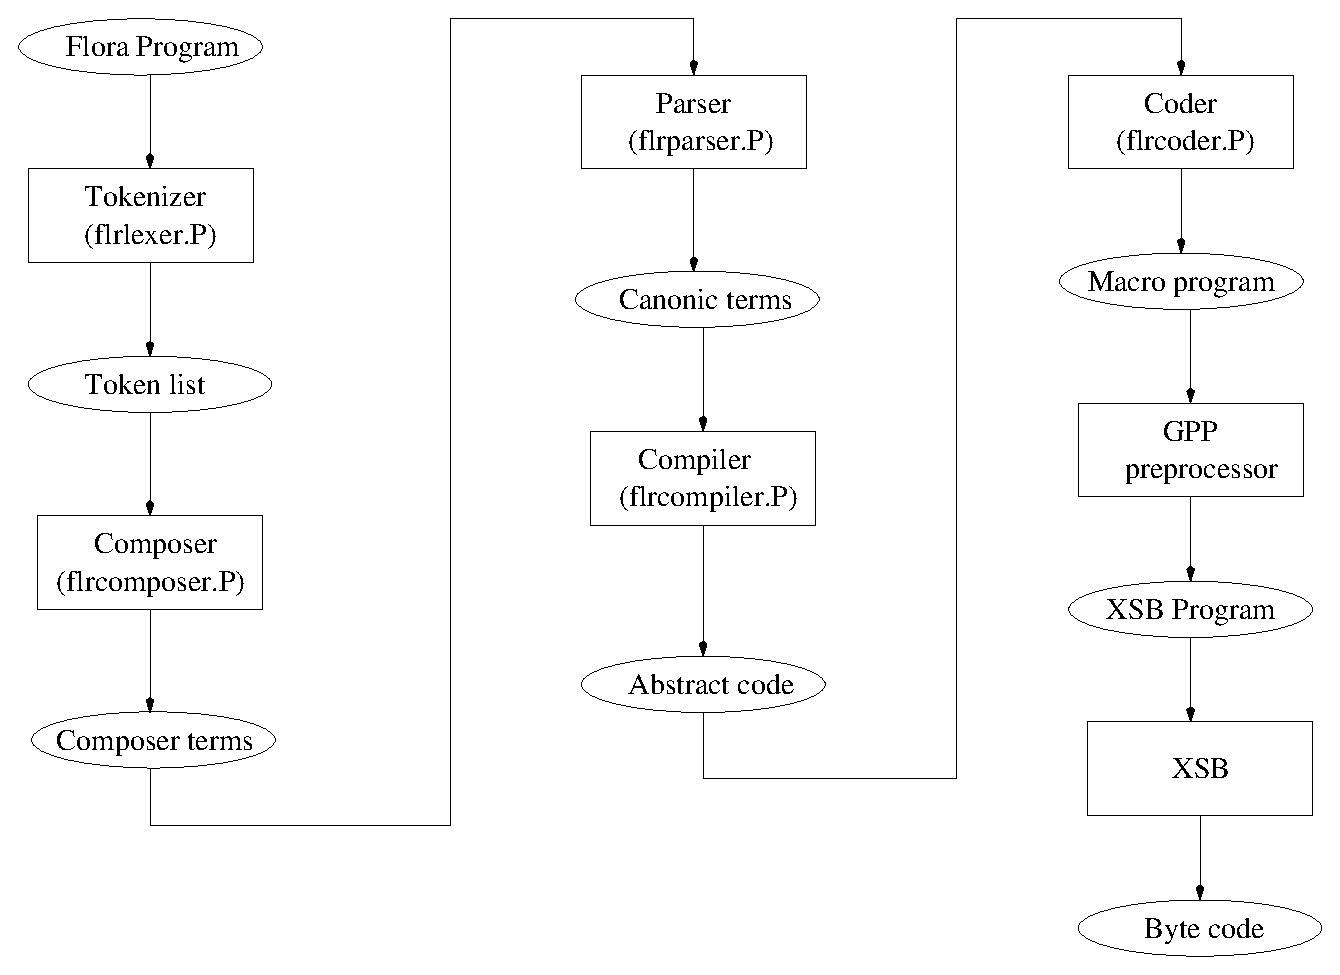
\includegraphics[width=5.5in]{architecture}
  \end{center}
  \caption{The architecture of the \FLORA system.}
  \label{fig-arch}
\end{figure}
%%

The following is a list of the key files of the system.
%%
\begin{itemize}
\item \texttt{flrshell.P}: The top level XSB module that implements the
  \FLORA shell --- a subsystem for accepting user commands and queries and
  passing them to the compiler.  See Section~\ref{sec-shell-commands} for a
  full description of shell commands.
\item \texttt{flrlexer.P}: The \FLORA tokenizer.
\item \texttt{flrcomposer.P}: The \FLORA composer, which parses tokens
  according to the operator grammar and does other magic.
\item \texttt{flrparser.P}: The \FLORA parser.
\item \texttt{flrcompiler.P}: The generator of the intermediate code.
\item \texttt{flrcoder.P}: The \FLORA coder, which generates XSB code.
\item \texttt{flrutils.P}: Miscellaneous utility predicates for loading
  programs, checking if files exist, whether they need to be recompiled,
  etc.
\end{itemize}
%%
Additional system libraries are located in the {\tt syslib/} subdirectory.
These include the various printing utilities, implementation for
aggregates, update primitives, and some others. The compiler determines
which of these libraries are needed while parsing the program. When a
library is needed, the compiler generates an {\tt \#include} statement to
include an appropriate file in the {\tt syslibinc} directory. For instance,
to include support for the {\tt avg} aggregate function, the compiler
copies the file {\tt syslibinc/flraggavg\_inc.flh} to the output {\tt .P}
file.  Since {\tt syslibinc/flraggavg\_inc.flh} contains the code to load
the library {\tt syslib/flraggavg.P}, this library will be loaded together
with that output file. The association between the libraries and the files
that need to be included to provide the appropriate functionality is
implemented in the file {\tt flrlibman.P}, which also implements the
utility used to load the libraries.

While {\tt syslib/} directory contains the libraries implemented in Prolog,
the {\tt lib/} directory contains libraries implemented in \FLORA itself.
Apart from that, the two types of libraries differ in functionality.  The
libraries in {\tt syslib/} implement the primitives that are part of the
syntax of the \FLORA language itself. In contrast, the libraries in {\tt
  lib/} are utilities that are part of the system, but not part of the
syntax. An example is the pretty-printing library.  Methods and predicates
defined in the libraries in {\tt lib/} are accessible through the {\tt
  @flora(lib-name)} system module and (unlike user modules) they are loaded
automatically at startup.

There are several subdirectories that hold the various files that contain
definitions included at compile time. These will be described in a
technical document.

A number of other important directories contain the various included files
(many of which include other files). The directory {\tt flrincludes/}
contains the all-important {\tt flora\_terms.flh} file, which defines all
the names used in the system. These names are defined as preprocessor
macros, so that it would be easy to change them, if necessary.
The directory {\tt genincludes/} currently contains the already mentioned
patch rules. The file {\tt flrpatch.fli} is a template, and {\tt
  flrpatch.flh}, which contains the actual patch rules, is generated from
{\tt flrpatch.fli} during the installation.

The directory {\tt includes/} contains the header file, which defines the
macros ({\it e.g.}, {\tt FLORA\_WORKSPACE}) that wrap all the names with
prefixes to separate the different modules of the user program.  The
directory {\tt headerinc/} is another place where the template files are
located. Each of these files contains just a few {\tt \#include}
statements, mostly for the files in the {\tt closure/} directory (which, if
you recall, contains pieces of the trailer). When the system is installed
certain combinations of these files are concatenated and dumped into the
{\tt trailer/} directory. Recall that the files in the {\tt trailer/}
directory are trailers that implement the closure axioms (there are three
trailers: without equality, with standard equality, and with \fl equality).
This double-indirection is needed to simplify the installation procedure
and to eliminate code duplication among the various trailers.

The directory {\tt p2h} contains (the only!) C program in the system. It
implements conversion of Prolog terms to HiLog and back. Finally, the {\tt
  pkgs/} directory is empty. Some day it will contain add-on programs, such
as Internet access, etc.



\bibliography{../../../docs/userman/manual}

\printindex

\end{document}
